%--------------------
% Packages
% -------------------
\documentclass[11pt,a4paper]{article}
\usepackage[utf8x]{inputenc}
\usepackage[T1]{fontenc}
\usepackage[english]{babel}
\usepackage{mathptmx}
\usepackage{xcolor}
% \usepackage{todonotes}
\usepackage{subcaption}
\usepackage[pdftex,linkcolor=black,pdfborder={0 0 0}]{hyperref}
\usepackage{graphicx}
\usepackage{calc}
\usepackage{enumitem}
\usepackage[a4paper, lmargin=0.1666\paperwidth, rmargin=0.1666\paperwidth, tmargin=0.1111\paperheight, bmargin=0.1111\paperheight]{geometry}
\usepackage[all]{nowidow}
\usepackage[protrusion=true,expansion=true]{microtype}
% \usepackage{parskip}

\frenchspacing
\linespread{1.2}

\newcommand{\leo}[1]{{\footnotesize \textcolor{blue}{$\ll$\textsf{Leonhard: #1}$\gg$}}}
\newcommand{\ms}[1]{{\footnotesize \textcolor{green}{$\ll$\textsf{Malte: #1}$\gg$}}}

\usepackage{listings, listings-rust}
\definecolor{codegreen}{rgb}{0,0.6,0}
\definecolor{codegray}{rgb}{0.5,0.5,0.5}
\definecolor{codepurple}{rgb}{0.58,0,0.82}

\makeatletter
\lstdefinestyle{mystyle}{
  frame=single,
  commentstyle=\color{codegreen},
  keywordstyle=\color{magenta},
  numberstyle=\tiny\color{codegray},
  stringstyle=\color{codepurple},
  basicstyle=\ttfamily\footnotesize,
  breakatwhitespace=false,         
  breaklines=true,                 
  captionpos=b,                    
  keepspaces=true,                 
  numbersep=5pt,                  
  showspaces=false,                
  showstringspaces=false,
  showtabs=false,                  
  tabsize=2}
\lstset{style=mystyle,language=Rust}
\makeatother

%-----------------------
% Begin document
%-----------------------
\begin{document}

% Title Page
\thispagestyle{empty}

\begin{center}
    \vspace*{1em}{\Huge An Expressive Query Interface for High-Fidelity Observability\par}
    
    \vspace*{1em}{\huge Richard Tang\par}
    
    \vspace*{3em}{\LARGE Advisor: Malte Schwarzkopf\par Reader: Ugur Cetintemel\par}
    
    \vspace*{12em}
\includegraphics[scale=0.08]{graphics/logo.png}\par
    \vspace*{1em}{\LARGE Department of Computer Science\par Brown University\par Providence, RI \par
    \today \par}
\end{center}
\newpage

\tableofcontents
\newpage

\section*{Acknowledgements}
\addcontentsline{toc}{section}{Acknowledgements}

TODO
% Thank you to Leonhard Spiegelberg for bringing me on board Tuplex in spring of 2021. Over the past
% three semesters, I had the amazing opportunity to work the project with Leonhard and learn about
% data science, systems, and research as a whole. Leonhard has offered guidance, support, and
% expertise on every step of this thesis, and I am so grateful for his mentorship.

% Thank you to my thesis advisor, Malte Schwarzkopf, for supporting me throughout my time working on
% Tuplex. Malte's attention to detail, prodding questions, and interest in my work helped me grow and
% kept me engaged throughout this process.

% Thank you to my reader, Shriram Krishnamurthi, for offering his systems expertise in reviewing my
% research. During my first semester at Brown in fall of 2018, Shriram's excitement, ability to
% engage, and passion catalyzed my interest in computer science when I took his introductory course.

% Finally, thank you to all of the professors, TAs, friends, and family who have supported me
% throughout my undergraduate experience at Brown. You have helped make these past four years so
% memorable and make it hard to finally say goodbye.

\newpage

\section*{Abstract}
\addcontentsline{toc}{section}{Abstract}

To understand the complex interactions in modern software, engineers often rely on detailed
\textit{high-fidelity telemetry} (HFT) data collected via instrumentation tools injected into the
kernel. Increasingly, developers have turned to eBPF (the extended Berkeley Packet Filter) for HFT
data collected, as it provides an extensible framework for high performance, low overhead
instrumentation. However, due to the eBPF's nascent, ever-evolving, and complex infrastructure,
developers often end up resorting to simple but inefficient programs, or a limited set of tools from
existing libraries.

% However, developers wishing to write eBPF programs immediately
% face significant obstacles: the
% ecosystem is volatile and constantly evolving, the documentation
% can be sparse or outdated, and
% developers must have a deep knowledge of not only the internal
% eBPF system architecture, but
% also the kernel tracing infrastructure and generally the kernel
% development environment. As a
% result, tracing programs are often simple and/or inefficient,
% incurring unnecessary (and
% sometimes prohibitive) overhead, and developers frequently resort
% to existing libraries like
% \texttt{bcc}/\texttt{bpftrace} that provide a limited set of
% tools.

We introduce eBQL, a novel eBPF streaming query engine that enables performant HFT data collection
via an expressive, high-level interface. eBQL provides a familiar relational layer over existing
kernel tracing infrastructure, allowing developers to query arbitrary kernel events with minimal
overhead. Internally, eBQL processes SQL queries into an abstract syntax tree (AST), analyzes and
optimizes the AST, then generates an eBPF program to execute the query, streaming output via a
structured schema definition.

We evaluate eBQL-generated eBPF programs on a RocksDB case study simulating a real-world workload.
eBQL queries incur a minimal abstraction overhead versus hand-optimized queries ($3.2\%$ vs.
$1.7\%$), and offer a $5-6\times$ performance improvement over a baseline eBPF program.

\newpage

\section{Introduction}

\subsection{Problem Statement}

As modern software continues to grow in complexity, observability and continuous monitoring is
becoming increasingful essential in ensuring a system's health and performance. To that end,
existing forms of telemetry data like metrics, logs, and traces provide valuable insights:
application-level logs on error messages and access patterns can aid in debugging software bugs and
identifying performance regressions; metrics on resource usage (e.g. CPU, memory, and I/O), tail
latencies, and uptime track overall health and reveal high-level anomalies in the system; and
distributed traces follow execution flow and identify bottlenecks within a request processing
pipeline.

Combined, these types of telemetry data---commonly called ``The Three Pillars of
Observability''---provide application-level monitoring of system health.  However, while this
telemetry data can reveal high-level \textit{symptoms} of system anomalies, there are often
insufficient to pinpoint the \textit{root cause}, as they lack the requisite granularity and thus do
not contain crucial information needed for debugging.

To analyze the root cause of performance regressions or system anomalies, developers must turn to
high-fidelity telemetry (HFT) data. HFT data is collected from kernel events with a much higher
level of granularity, and provides detailed contextual information at the triggered trace event.
Using HFT data, developers can interactively investigate various system events for anomalies, and
identify the root cause for system anomalies.

However, actually generating HFT data can be highly involved, and the existing kernel functionality
can be inflexible and/or inefficient, as tracing infrastructure often relies on costly
interrupt-based event instrumentation, requires extensive kernel knowledge in order to develop
efficient and sound programs, and sometimes necessitates kernel patches. Especially since this
functionality is often injected at program hot paths or in systems under high load, HFT data
collection programs \textit{must} incur negligible overhead and remain performant, even under
intense resource pressure. Moreover, due to the ever-evolving nature of distributed applications,
data collection programs must be dynamic and flexible.

Recently, the growth and development of eBPF (the extended Berkeley Packet Filter), a kernel
subsystem, has enabled an extensible interface for dynamic kernel tracing. eBPF provides a sandboxed
virtual environment to run statically verified custom user ``probes'' that can perform in-kernel
processing and context-specific information retrieval. These probes are then run at user-specified
events, from kernel tracepoints and kprobes to the network ingress/egress path.

Unfortunately, like kernel tracepoints, eBPF program development can be prohibitively complex, as
developers must grapple with not only the kernel infrastructure, but now also subtleties in the eBPF
architecture (and in particular, the BPF program verifier). Without a thorough knowledge of eBPF and
the kernel as a whole, developers are often stuck writing simple but inefficient programs, or
resorting to a set of existing, but limited and unstructured, tools (e.g. from
\texttt{bcc}/\texttt{bpftrace}).

\subsection{eBQL}

To ease HFT data collection, we propose eBQL, an eBPF streaming query engine with an expressive
interface that analyzes queries and generates optimized eBPF programs. At a high level, eBQL takes
in an input query, parses it into an abstract syntax tree (AST), generates an optimal physical plan
consisting of an kernel-space (i.e. eBPF) event processing component and a user-space component that
additionally processes kernel events, before emitting to an output destination.

eBQL has three design goals:
\begin{enumerate}
        \item \textbf{Provide an expressive query interface} for application developers to
            dynamically query for HFT data at a high level, abstracting away internal eBPF
            implementation details such that a deep knowledge of eBPF or the kernel is not required.
        \item \textbf{Expose a general, structured API} for generated HFT data to enable seamless
            integration with streaming data analytics pipelines like Spark or Flink, or existing
            observability systems like Mach or M3DB.
        \item \textbf{Facilitate performance optimizations} by providing a centralized system for
            identifying optimal user-kernel space transitions in physical plans, analyzing physical
            plans across probes to limit redundancy, and enabling stateful synopsis sharing between
            different probes.
\end{enumerate}

We implement an eBQL prototype in Rust, and evaluate its performance on a simulated RocksDB
workload. We find that eBQL's abstraction layer incurs only minimal---and resolvable---overhead over
hand-optimized eBPF programs ($3.2\%$ vs $1.7\%$), and outperforms existing methods of eBPF-based
HFT data collection by $5-6\times$.

In summary, this thesis makes the following contributions:
\begin{enumerate}
    \item We define a \textbf{query language} over existing kernel event streams, associating events
        with a structured relation, and extending SQL to support streaming semantics.
    \item We \textbf{dynamically generate and load eBPF code} in a composible way from a physical
        plan that was parsed and analyzed from an input query.
    \item We \textbf{analyze the feasibility and performance implications} of query physical plan
        implementations in eBPF contexts, and investigate the optimal user-kernel work division.
\end{enumerate}

% References:
% \begin{itemize}
    % \item RocksDB
    % \item perf
    % \item ftrace
    % \item tracepoints
    % \item eBPF
    % \item bcc
    % \item bpftrace
    % \item Spark
    % \item Flink
    % \item Mach
    % \item M3DB
% \end{itemize}




\section{Background and Related Work}

\subsection{Observability}

As software continues to scale into Internet-scale systems that have complex interactions with other
applications and underlying hardware, so too does their failure domain: distributed systems become
pathologically unpredictable, as performance regressions and partial failures can arise anywhere
from the network \ref{8-fallacies} to the underlying storage system to competing
processes on the same machine \ref{noisy-neighbors}. Thus, in order to develop and maintain robust
systems, developers increasingly rely on observability systems to monitor system health and
performance (ref: DSO) (ref: SRE book).

\subsubsection{Existing Systems}

Current observability systems focus primarily on three types of telemetry data: logs, metrics, and
traces (collectively termed the ``Three Pillars of Observability'' (ref: pillars of observability)):

% TODO: maybe condense this a lot?
\begin{itemize}
    \item Logs are semi-structured or unstructured strings added into applications by developers to
        expose highly granular information with local context. For example, logs could include stack
        traces from software bugs or exceptions, or database access events with associated contexts
        to debug performance regressions. Existing systems include ElasticSearch (ref: ES) and CLP
        (ref: CLP) for log processing.
    \item Metrics provide quantitative measurements of system performance and availability at a
        specific point in time. Metrics can be \textit{counters} that represent cumulative,
        monotonically increasing values (e.g. HTTP requests received, GC collections executed),
        gauges to model system state (e.g. CPU/memory usage, machine availability), or histograms of
        observed values (e.g. request latencies) (ref: metric types). Existing systems include
        Prometheus (ref: Prometheus) and M3DB (ref).
    \item Distributed traces follow program execution flow and often resemble call graphs. For
        example, a trace of an HTTP request might show the internal backend and database functions
        invoked to satisfy the request. Existing systems include Jaeger (ref: Jaeger) and Zipkin
        (ref: Zipkin).
\end{itemize}

Current observability systems have expanded into robust distributed systems themselves, with some
like InfluxDB (ref) and ClickHouse (ref) capable of handling general time-series data. However,
these systems often fail to capture the underlying root cause of a system anomaly (ref: doordash bpf).

Concretely, consider a performance engineer investigating a performance regression in a
microservices application. Via application-level aggregated metrics, the engineer can identify a
system bottleneck from the backing RocksDB application by identifying spiking tail latency metrics;
from there, they can use traces to pinpoint the specific problematic function (say, \texttt{pread64}
within the \texttt{GET} operation). However, although the engineer now knows \textit{where} the
system bottleneck arises, they do not know \textit{why} it is occuring. 

To analyze the root cause of performance regressions like this, developers must turn to
high-fidelity telemetry (HFT) data.

\subsubsection{High-Fidelity Telemetry (HFT) Data}

HFT data refers to data generated from kernel events with a much higher level of granularity; some
examples are page cache evictions or CPU scheduler events. As HFT data is generated within the
kernel, they contain comprehensive information about the context from which it originated, such as
the specific inode and device number on which a page cache eviction occurs, or which \texttt{pid}s
are being scheduled and their priority levels. Using HFT data, developers can interactively
investigate various system events for anomalies, and identify the root cause for system anomalies.

The amount of HFT data available to be collected can be orders of magnitude greater than that of
traditional telemetry data, due to the higher granularity of each individual data point. As an
illustrative example, in a RocksDB application, gathering HFT data on \texttt{pread64} syscall
\textit{invocations} alone can produce millions of events per second; the amount could significantly
increase if other events were instrumented (such as CPU scheduling, page cache events, or memory
allocations). As such, HFT data is often summarized as some aggregate statistic, such as average,
histogram buckets, or quantiles.

HFT data can prove invaluable in identifying performance regressions. In the above example, an
engineer can use HFT data to formulate a hypothesis about the root cause, and monitor various kernel
events. For instance, they could correlate system call latency with other kernel events like page
cache events, and identify that a competing process is causing repeated page cache evictions; from
then, they can appropriately handle the competing process (e.g. by re-scheduling it to a different
machine).

HFT data collection's use case of anomaly debugging imposes strict requirements. Especially since
this functionality is often injected at program hot paths or in systems under high load, HFT data
collection programs must incur negligible overhead and remain performant, even under intense
resource pressure. Moreover, due to the ever-evolving nature of distributed applications, programs
must be dynamic, flexible, and simple to generate. In addition, HFT data must be as complete as
possible, as sparse data sampling can result in key anomalous events frequently being dropped (ref:
sampling bad). Finally, HFT data output should be exposed through accessible interfaces, as often
their results must be post-processed for offline analysis.

To support HFT data collection, various tracing technologies have been developed, either within the
Linux kernel or as research systems. However, these tools often introduce prohibitive overhead, emit
insufficient contextual information, or are difficult to develop and adapt, making it unsuitable to
handle HFT data collection's requirements.

Event profilers like \texttt{perf} (ref), \texttt{ftrace} (ref), \texttt{DTrace} (ref), and
\texttt{SystemTap} trace kernel events and emit information at various degrees of granularity.
However, these systems often incur prohibitive overhead costs that make them unsuitable for
production systems (ref: function duration with ftrace, Hubble paper). For example, the
\texttt{perf} subsystem uses interrupt-based sampling, which introduces costly context switches and
branch misses (ref: perf tutorial, perf analysis modern CPUs). These systems must thus resort to
aggressive sampling, causing key events to be dropped. Moreover, these utilities emit data in ad-hoc
formats, forcing developers to write custom post-processing scripts and manually manage result
storage.

Other tracing instrumentation tools like Magpie (ref), KUTrace (ref), Nanoscope (ref), Shim (ref),
and Hubble (ref) generate HFT data through lightweight instrumentation. Although these systems are
performant, they are purpose-specific: Nanoscope and Hubble specifically target the Android runtime,
KUTrace is a Linux kernel tracing patch, and Shim primarily targets hardware performance counters
and signals. As a result, they are not suitable for general-purpose application tracing, and
interacting with the generated data also requires manual post-processing.

The Linux kernel exposes tracepoints (ref) and kprobes (ref), allowing developers to instrument
specific kernel instructions or events with low overhead. However, regular tracepoints can only be
interacted with by writing user-space code to process a pre-determined context, and kprobes
introduce significant safety risks, as faulty programs could crash the kernel (ref: guts of
kprobes). Both solutions require developers to intimately understand the kernel tracing
infrastructure.

The fragmentation of various tracing utilities and output formats poses real difficulties for
developers trying to debug anomalies. In a case study by Cloudflare (ref: blog 1, blog 2) debugging
a latency spike, five separate custom \texttt{SystemTap} scripts were required, alongside
\texttt{netstat} and \texttt{tcpdump}, in order to identify the root cause. Without a structured
utility to process results, developers are forced to manually inspect and debug system regressions.

\subsection{eBPF}

In recent years, a novel kernel technology, the extended Berkeley Packet Filter (eBPF), has opened
a promising new approach to HFT data collection by providing a minimalistic sandboxed ``virtual
machine'' (ref: eBPF VM patch, tc classifier programmable) to safely execute custom user programs,
allowing developers to safely and efficiently extend kernel capabilities without kernel patches or
modules (ref: what is eBPF).

The Berkeley Packet Filter (BPF or cBPF), introduced in 1992, originated as a subsystem that allowed
userspace programs to execute in a limited kernel virtual machine at specific network stack hook
points (ref: BSD packet filter). Its functionality was later expanded into its current state, eBPF,
with an expanded instruction set architecture that closely maps to native CPU instructions, a JIT
compiler, a verifier to ensure program safety, persistent state via BPF maps, and support for the
LLVM toolchain for compilation (ref: what is eBPF). Most importantly, eBPF expanded to arbitrary
kernel events, allowing custom programs to hook into events ranging from the network stack, to Linux
Security Modules (LSM), to internal tracing technologies, such as (raw) tracepoints,
\texttt{u[ret]probes/k[ret]probes}, and \texttt{fentry/fexit}. This expanded feature set has enabled
highly performant and extensible HFT data collection. (Beyond tracing, eBPF has also been used for
efficient in-kernel packet processing (ref: XDP), CPU scheduling (ref: Ghost), and kernel bypass
storage functions (ref: XRP)).

\begin{quote}
From here on, the term ``eBPF'' will be used interchangeably with ``BPF'', as cBPF is no longer
used.
\end{quote}

\subsubsection{eBPF System Architecture}

\begin{figure}[htpb]
    \centering
    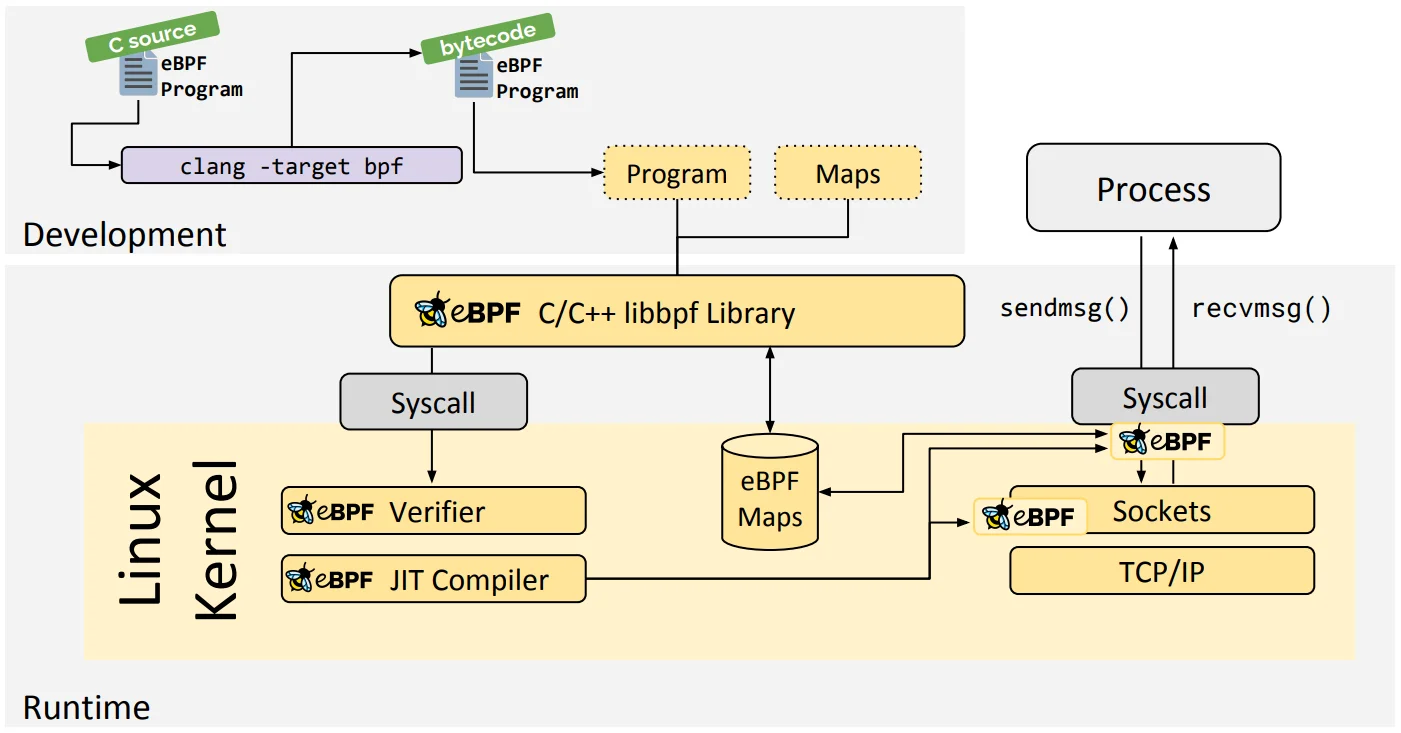
\includegraphics[width=0.8\textwidth]{diagrams/ebpf-architecture.png}
    \caption{eBPF Architecture using libbpf (from (ref: what is eBPF))}
    \label{fig:bpf-arch}
\end{figure}

eBPF consists of multiple components (see Figure \ref{fig:bpf-arch}):

\begin{itemize}
    \item Engineers write custom eBPF program code in essentially a subset of C, albeit with
        important exceptions: for example, unbounded or dynamically sized loops are forbidden,
        helper function calls could not have more than 5 arguments (non-inlined helper functions
        were not supported until Linux v4.9 (ref: bpf function calls)), the stack size is restricted
        to 512 bytes, and a maximum of 1 million BPF instructions are allowed (prior to Linux v5.1,
        this limit was a mere 4096 instructions (ref: increase complexity limit)). eBPF C disallows
        dynamic memory; instead, developers must use BPF maps to persist state across program
        executions or use memory beyond the 512B limit. BPF maps also enable communication between
        user and kernel space. eBPF source code files can contain multiple eBPF ``programs'' for
        different kernel events, specified with a \texttt{SEC} macro before function definitions.

        As an example, Figure \ref{code:pread64-unopt} contains a standard BPF program to instrument
        the \texttt{pread64} system call.
\begin{figure}
\begin{lstlisting}[language=C]
#include "vmlinux.h"
#include <bpf/bpf_core_read.h>
#include <bpf/bpf_helpers.h>
#include <bpf/bpf_tracing.h>

typedef struct {
    u64 time;
    u64 fd;
    u64 cpu;
    u64 count;
} raw_pread_t;

#define RB_MAX_ENTRIES (1024 * sizeof(raw_pread_t))
struct {
    __uint(type, BPF_MAP_TYPE_RINGBUF);
    __uint(max_entries, RB_MAX_ENTRIES);
} ring_buf_pread_query SEC(".maps");

SEC("tp/syscalls/sys_enter_pread64")
u32 pread_query(struct trace_event_raw_sys_enter* ctx) {
    raw_pread_t* q = bpf_ringbuf_reserve(
        &ring_buf_pread_query,
        sizeof(raw_pread_t),
        0
    );
    if (!q) {
        bpf_printk("failed to allocate space in ring buffer");
        return 1;
    }
    q->time = bpf_ktime_get_ns();
    q->fd = ctx->args[0];
    q->cpu = bpf_get_smp_processor_id();
    q->count = ctx->args[2];
    bpf_ringbuf_submit(q, 0);
    return 0;
}

char LICENSE[] SEC("license") = "Dual BSD/GPL";
\end{lstlisting}
\caption{A standard \texttt{pread64} tracing BPF program.}
\label{code:pread64-unopt}
\end{figure}

        Once written, these programs are compiled into eBPF bytecode using the LLVM/\texttt{clang}
        toolchain, which generates an object file containing all defined eBPF programs and map
        definitions. 

    \item When the program is ready to be inserted into the kernel, eBPF bytecode is passed to the
        \texttt{bpf} system call (ref: bpf system call), which loads the program into the kernel. As
        the \texttt{bpf} syscall operates on compiled program bytes, working with compiled programs
        can prove difficult (e.g. to edit global variables or map definitions before runtime); thus,
        a higher-level wrapper library, \texttt{libbpf}, was introduced (in the figure, the
        higher-level \texttt{libbpf} library is for C/C++; however, support for other languages,
        like Go and Rust, also exist).

    \item The \texttt{bpf} syscall passes the eBPF bytecode to the eBPF verifier, which ensures the
        safety and soundness of eBPF programs, rejecting any program that might potentially be
        unsound by checking for guaranteed termination and memory safety. The verifier traverses
        through all program paths, using heuristics to prune potential program branches (ref: static
        analysis), and maintaining a DAG to ensure bounded loop termination and other CFG validation
        (ref: linux eBPF verifier doc). On each instruction, the verifier maintains a range of
        possible values for each register value, ensuring that they are valid (e.g. a memory access
        for register $R$ is in the allowed range). Only after verifying that all program
        instructions are sound does the kernel accept the eBPF program.

        Because dynamic memory access adds significant complexity, the eBPF verifier requires that
        such access is known at verification time. In particular, BPF maps, stored in kernel space
        and represented with file descriptors, must have their \texttt{fd}s embedded in the
        \texttt{BPF\_LD\_IMM64} instruction; and function calls must be to either a constant
        function definition or a pre-defined BPF ``helper function'' (ref: bpf helpers) that exposes
        additional kernel functionality (in other words, function pointers are disallowed in BPF
        programs, except in certain contexts like in the \texttt{bpf\_for\_each\_map\_elem} helper).
    \item After verification, the program is injected into the designated hook point; then, every
        time the kernel event occurs, the program runs within that context. BPF programs then
        communicate with userspace programs by writing data to the shared BPF maps, on which
        userspace programs can then invoke syscalls to retrieve the data from the kernel.
\end{itemize}

\subsubsection{eBPF as a HFT Data Collection Tool}

Given its architecture, eBPF is uniquely suited to handle HFT data collection. 

First, the eBPF verifier guarantees that custom programs are safe to run, and that users have
requisite permissions. Thus, buggy or unsafe programs are rejected before being loaded and executed.
This exists in stark contrast to existing technology, where software bugs can crash the entire
kernel. For example, it is possible to hook into arbitrary kernel instructions for tracing via
kprobes (ref: kprobes), but errors in the probes would crash the kernel (ref: guts of kprobes).

Second, expressive eBPF programs can run with high performance, minimal overhead, at a level
acceptable in production environments. Because eBPF programs are provably sound, they can inject
\textit{custom} code into exclusive kernel tracing infrastructure, like
\texttt{fentry}/\texttt{fexit} and tracepoints (which do not offer the same expressiveness to other
userspace tracing methods). Moreover, the eBPF JIT compiler transparently compiles eBPF bytecode
into native machine instructions, allowing cross-platform efficient execution with almost trivial
overhead. As a concrete example, BPF programs attached to the XDP hook point can process over 24
million packets per second (ref: XDP).

Third, eBPF programs can be dynamically loaded and modified during application runtime, allowing
instrumentation without disrupting existing systems. As applications evolve and change, eBPF
programs can be seamlessly modified to accommodate the new changes; similarly, the programs
themselves may be extended with additional functionality without disrupting existing systems. This
allows teams to decouple application development and monitoring, lifting the burden off engineers
during the development process.

\subsection{eBPF Development Challenges}

Despite its various benefits, onboarding into the eBPF ecosystem and developing performant,
verifiable eBPF programs remains a significant challenge.

First and foremost, the eBPF verifier can reject seemingly sound BPF programs. In some cases, the
verifier is overly restrictive, rejecting programs due to an inability; in other cases, the verifier
encounters constructs outside of eBPF's current supported feature set, causing it to reject
programs. To complicate matters, the verifier's error messages deal primarily with eBPF bytecode and
the virtual registers, and can be uninformative at best and misleading at worst. We consider three
illustrative examples:

\begin{enumerate}
    \item The eBPF program in Figure \ref{code:fail-1} accumulates up to
        \texttt{RINGBUF\_MAX\_ENTRIES} context values, then emits them to the ring buffer.
\begin{figure}[htpb]
\begin{lstlisting}[language=C]
#include "vmlinux.h"
#include <bpf/bpf_core_read.h>
#include <bpf/bpf_helpers.h>
#include <bpf/bpf_tracing.h>
#define RB_MAX_ENTRIES (1<<18)
struct {
    __uint(type, BPF_MAP_TYPE_RINGBUF);
    __uint(max_entries, (RB_MAX_ENTRIES * sizeof(u64)));
} rb SEC(".maps");
u64 global_count = 0;

SEC("tp/syscalls/sys_enter_pread64")
u32 pread_query(struct trace_event_raw_sys_enter *ctx) {
    u64 count = global_count;
    global_count += 1;
    if (count >= RB_MAX_ENTRIES) {
        u64 *records = bpf_ringbuf_reserve(&rb,
            count * sizeof(u64), 0);
        if (records != NULL) {
          bpf_ringbuf_submit(records, 0);
        }
        global_count = 0;
    }
    return 0;
}
\end{lstlisting}
\caption{An example program that accumulates values before emitting to user-space.}
\label{code:fail-1}
\end{figure}

    This fails the eBPF verifier with the error: 
\begin{lstlisting}
// ... more output ... //
R1_w=inv262144 R2_w=inv(id=0,umin_value=262144) R10=fp0
; u64 *records = bpf_ringbuf_reserve(&rb, count*sizeof(u64), 0);
7: (67) r2 <<= 3
8: (b7) r6 = 0
12: (85) call bpf_ringbuf_reserve#131
R2 is not a known constant'
\end{lstlisting}
    From a developer standpoint, we can verify that the BPF program is safe to execute, as
    \texttt{global\_count} will only ever be at most \texttt{RB\_MAX\_ENTRIES}; and because we
    assign \texttt{global\_count} to a local variable \texttt{count}, this would not pose an issue
    with other concurrently executing processes. However, because the verifier operates on variable
    ranges with only individual execution-level context, it is unable to verify the logic.

    To remedy this, a line manually setting \texttt{count = RB\_MAX\_ENTRIES} would be required.
    This kind of massaging to appease the verifier is common in eBPF programs.

    \item The eBPF code snippet in Figure \ref{code:fail-2} attempts to copy over data from one
        buffer to another (both stored as global variables).
\begin{figure}[htpb]
\begin{lstlisting}[language=C]
#define BUF_SZ (1 << 16)
u8 src[BUF_SZ] = {0};
u8 dst[BUF_SZ] = {0};
// ... additional code ... //
__builtin_memcpy(dst, src, sizeof(src));
\end{lstlisting}
    \caption{An eBPF code snippet that copies values from one eBPF array to another.}
    \label{code:fail-2}
\end{figure}
    On program load, the BPF verifier emits the message, \texttt{error: A call to built-in
    function 'memcpy' is not supported}, and rejects the program, even though the clang instrinsic
    \texttt{\_\_builtin\_memcpy} is supported in eBPF environments. After much digging, the cause of
    this error is because the stack size is limited to 512B, and so builtin memory operations fail
    when operating on structs larger than that (ref: iovisor bcc memset).

    To remedy this, the \texttt{memcpy} would have to be replaced with a call to
    \texttt{bpf\_probe\_read\_kernel}, which introduces an additional overhead of memory copying and
    runtime safety checks.

    \item The eBPF code snippet in Figure \ref{code:fail-3} attempts to declare a map of $2^{20}$
        elements.
\begin{figure}[htpb]
    \centering
\begin{lstlisting}[language=C]
struct {
    __uint(type, BPF_MAP_TYPE_HASH);
    __type(key, u64);
    __type(value, u64);
    __uint(max_entries, (1 << 20));
} map SEC(".maps");
\end{lstlisting}
    \caption{An eBPF code snippet attempting to initialize a large map.}
    \label{code:fail-3}
\end{figure}

    On program load, the BPF verifier emits the error message:
\begin{lstlisting}
Error in bpf_create_map_xattr(prog.bss):Argument list too long(-7). Retrying without BTF.
map 'prog.bss': failed to create: Argument list too long(-7)
libbpf: failed to load object 'prog_bpf'
libbpf: failed to load BPF skeleton 'prog_bpf': -7
\end{lstlisting}

    After much investigation, the root cause for this is because \texttt{bpf\_create\_map} invokes
    the internal kernel \texttt{kmalloc} (ref: kernel code), which on most machines has a limit of
    4MB; thus, maps larger than that are rejected. Unfortunately, the actual error message provides
    little insight into BPF's limitations, with no specific indication that map sizes have this
    fixed limit.
\end{enumerate}

There are some important takeaways from this. First, due to the verifier's limited
individual-execution scope, developers must frequently appease the verifier by adding redundant
checks and redundant accesses, incurring real performance hits; otherwise, sound programs would be
rejected. Second, the verifier often emits obscure or misleading error messages, forcing the
developer to manually test different parts of their program, scour online discussion forums, or
investigate the BPF kernel itself to pinpoint the cause. These combined can significatly impedes
developer workflows.

Beyond the verifier, the eBPF ecosystem also can hinder developers. Due to its volatile and evolving
interface, many APIs are unstable and are frequently changed; moreover, online documentation often
fails to keep up with recent developments, resulting in misleading and outdated information, or even
a complete lack thereof, forcing developers to resort to kernel patch updates or mailing lists. As
concrete examples, the \texttt{bpf-helpers} manpage explicitly refers developers to the kernel
source for an up-to-date list of helper functions (ref: bpf-helpers manpage); and simple questions
such as ``Can I clear a BPF map within a BPF program?'', ``How can I pin BPF maps to share across
programs?'', and ``Can I use this BPF helper function at this kernel event?'' require deep
exploration of online resources or even the kernel source (ref: pin patch, iovisor-dev mailing
list).

Even with a BPF program that passes the BPF verifier, developers must also be familiar with kernel
environments, which operate with further restrictions (for instance, floating point operations are
not supported). Moreover, due to the eBPF architecture, it is easy to develop inefficient programs
without a deep knowledge of eBPF subtleties.

For example, prior work (ref: eBPF traffic sketching) has explored different memory access patterns
in eBPF for data structure design, comparing four different ways to represent a 2D $R\times C$ array
(an array map with one $R\times C$-sized array, an array map with $R$ entries of $C$-sized arrays,
an array map with $R\times C$ entries, and an array of array map with $R$ array maps, each with $C$
entries). Perhaps surprisingly, different access patterns incur varying amounts of overhead (Figure
\ref{fig:array-access}).

\begin{figure}[htpb]
    \centering
    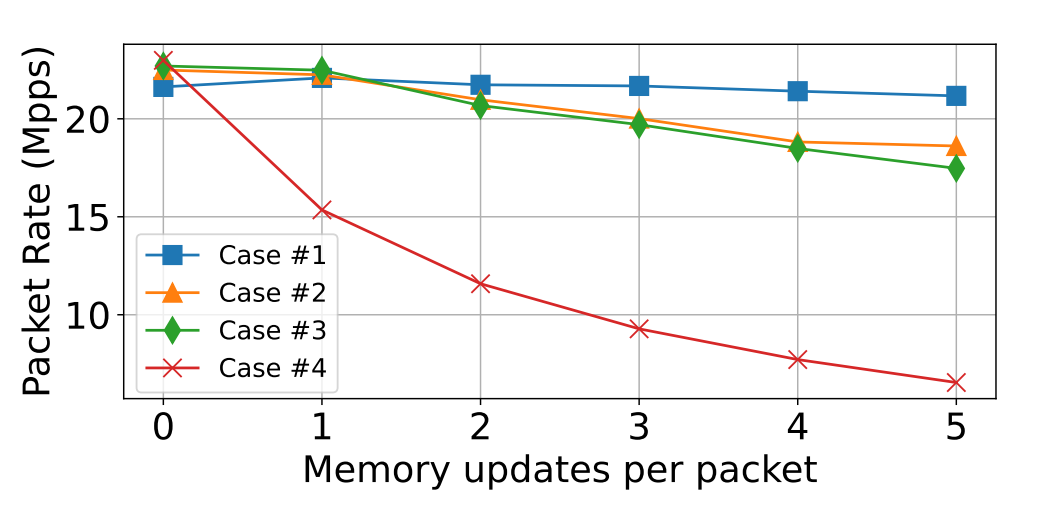
\includegraphics[width=0.8\textwidth]{diagrams/ebpf-array-accesses.png}
    \caption{Different methods of array accesses (from (ref: eBPF traffic sketching)).}
    \label{fig:array-access}
\end{figure}

Beyond these cases, eBPF structures often incur hidden synchronization overhead due to its
concurrent execution environment; this can be resolved with different per-CPU and task-local
constructs that reduce overhead at the expense of higher developer complexity, but only if
developers are intimately aware with the environment (ref: fast and slow blogpost).

\subsection{Related Work}

To ease BPF development, a robust ecosystem providing higher-level wrappers around BPF internals has
emerged.

\subsubsection{\texttt{bcc}}

One of the most popular development frameworks is the BPF Compiler Collection, or \texttt{bcc} (ref:
bcc). Its architecture is displayed in Figure \ref{fig:bcc-architecture}.

\begin{figure}[htpb]
    \centering
    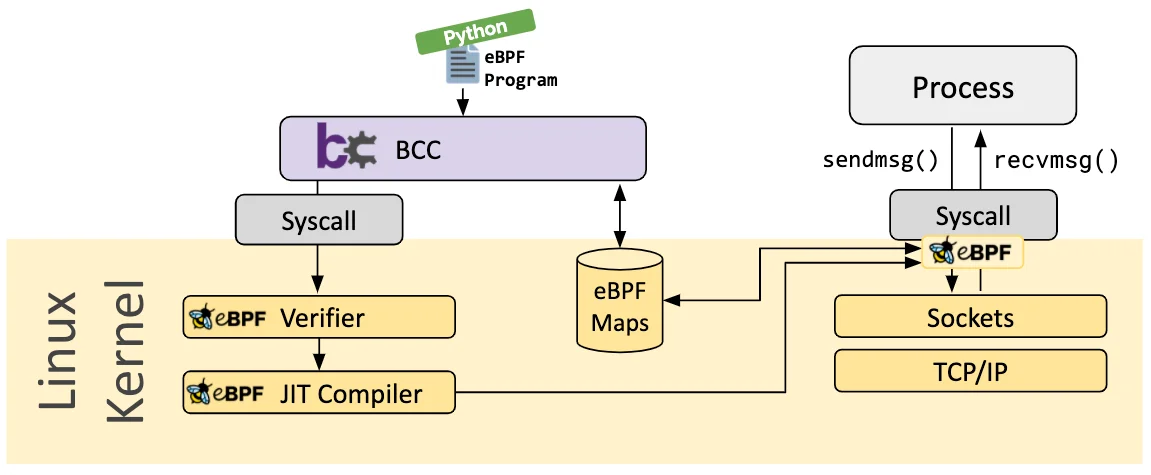
\includegraphics[width=0.8\textwidth]{diagrams/bcc-architecture.png}
    \caption{The BCC eBPF Architecture.}
    \label{fig:bcc-architecture}
\end{figure}

Development follows a similar workflow to raw BPF program development, with some key additions:
\begin{itemize}
    \item \texttt{bcc} introduces a higher-level Python/Lua frontend for communicating with BPF
        programs and the \texttt{bpf} syscall, simplifying access and modification of shared BPF
        maps, global variables, and other program configuration options.
    \item \texttt{bcc} adds additional macros and pre-processing steps before loading BPF code,
        simplifying section/program type macros, map definitions and accesses, and certain BPF
        helper functions.
\end{itemize}

Despite its simplified development environment, however, \texttt{bcc} runs into numerous challenges.
First, although some constructs are simplified, the actual BPF program---the key instrumentation
code---must still be written in BPF C; the program text must then be embedded into the Python
frontend and loaded, before the program can begin tracing. For example, the BCC program in Figure
\ref{code:bcc-example} (from (ref: disksnoop)) traces disk block IO requests.
\begin{figure}[htpb]
\begin{lstlisting}[language=C]
# load BPF program
b = BPF(text="""
#include <uapi/linux/ptrace.h>
#include <linux/blk-mq.h>

BPF_HASH(start, struct request *);

void trace_start(struct pt_regs *ctx, struct request *req) {
    u64 ts = bpf_ktime_get_ns();
    start.update(&req, &ts);
}

void trace_completion(struct pt_regs *ctx, struct request *req) {
    u64 *tsp, delta;
    tsp = start.lookup(&req);
    if (tsp != 0) {
        delta = bpf_ktime_get_ns() - *tsp;
        bpf_trace_printk("%d %x %d\n",
            req->__data_len, req->cmd_flags, delta / 1000);
        start.delete(&req);
    }
}
""")

b.attach_kprobe(event="blk_start_request", fn_name="trace_start")
b.attach_kprobe(event="blk_account_io_done", fn_name="trace_completion")
// Additional processing code...
\end{lstlisting}
\caption{A BCC \texttt{disksnoop} script (from (ref: disksnoop))}
\label{code:bcc-example}
\end{figure}

The fundamental burden of developing the BPF code is still the developer's responsibility.
Furthermore, \texttt{bcc}'s various abstractions can additionally hinder development, as it uses its
own naming conventions, hides various initialization and auto-generated struct definitions, and uses
a non-standard object-oriented version of C that often differs from internal kernel operations (ref:
bcc to libbpf). As a result, the standard \texttt{libbpf} development environment is often
preferred.

\subsubsection{Cilium}

Cilium is a cloud-native monitoring, networking, and security platform for managing containerized
Kubernetes environments (ref: Cilium). Cilium provides useful utilities out-of-the-box, exposing
Prometheus metrics for container and pod health, and abstracts away much of the complexity of eBPF
by using it only internally. 

However, its focus is on cloud, containerized environments, with functionality geared primarily
towards networking and security; as such, its monitoring utilities are mainly for those purposes,
and due to its higher-level nature, exposes more aggregate metrics on system health, rather than the
high-granularity HFT data needed for root cause analysis.

In addition to the Cilium platform, it provides a Go frontend wrapping eBPF functionality (much like
\texttt{bcc}), simplifying management of BPF maps and programs from user-space. However, like
\texttt{bcc}, Cilium also relies on embedded eBPF programs. Thus, the burden of developing BPF
instrumentation programs still lies with the developer.

\subsubsection{\texttt{bpftrace}}

\texttt{bpftrace} (ref: bpftrace) provides the most high-level interface over eBPF, exposing a
tracing language similar to DTrace (ref: DTrace). Its architecture is displayed in Figure
\ref{fig:bpftrace-architecture}.

\texttt{bpftrace} takes in a script written in its higher-level language, parses it into an AST,
converts it into LLVM IR, then hooks into the LLVM toolchain to compile into eBPF bytecode. The
compiled program is then automatically loaded into the kernel.

\begin{figure}[htpb]
    \centering
    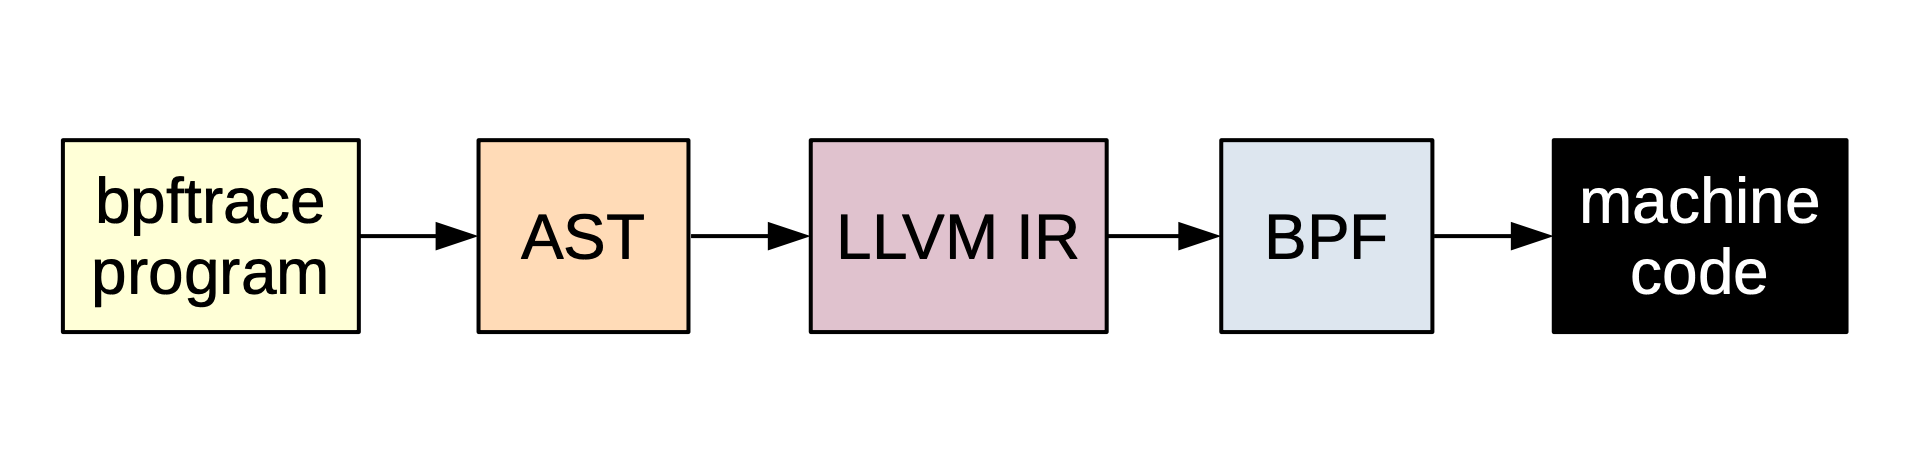
\includegraphics[width=0.8\textwidth]{diagrams/bpftrace-architecture.png}
    \caption{\texttt{bpftrace} architecture (from (ref: BPF Internals))}
    \label{fig:bpftrace-architecture}
\end{figure}

\texttt{bpftrace}, in many ways, provides a sufficiently high-level abstraction over BPF, enabling
developers to write custom tracing scripts without writing BPF C. However, its design contains
two problems. First, \texttt{bpftrace} is a fundamentally procedural language; thus, developers must
explicitly enumerate program steps, grounding development into the same procedural
programming required for BPF C.

Concretely, consider the \texttt{bpftrace} program in Figure \ref{code:bpftrace-ex}, which
instruments the \texttt{open} syscall.

\begin{figure}[htpb]
\begin{lstlisting}[language=C]
tracepoint:syscalls:sys_enter_open,
tracepoint:syscalls:sys_enter_openat
{
    @filename[tid] = args.filename;
}
tracepoint:syscalls:sys_exit_open,
tracepoint:syscalls:sys_exit_openat
/@filename[tid]/
{
    $ret = args.ret;
    $fd = $ret >= 0 ? $ret : -1;
    $errno = $ret >= 0 ? 0 : - $ret;
    printf("%-6d %-16s %4d %3d %s\n", pid, comm, $fd, $errno,
            str(@filename[tid]));
    delete(@filename[tid]);
}
END
{
    clear(@filename);
}
\end{lstlisting}

    \caption{The bpftrace \texttt{opensnoop.bt} script (ref: opensnoop)}
    \label{code:bpftrace-ex}
\end{figure}

In this code example, the developer is responsible for operating on the arguments in a C-like
manner, and must manually manage BPF map state; thus, although the requirements for BPF development
have been lowered given its higher-level interface, developers must still understand how BPF maps,
tracepoints, and program types work.

\subsection{Streaming Data Management}

Before presenting eBQL's architecture, we briefly explore streaming data management. Because eBPF
programs are invoked only when a kernel event occurs, the resulting output models a data stream,
where an unbounded, continuous set of data is streamed from the kernel.

Formally, a data stream is a real-time, continuous, ordered (in eBPF, explicitly by timestamp)
sequence of items (ref: issues in data stream management pdf). Queries over data streams thus run
continuously over a period of time, and incrementally return new results as new data arrive; these
are known as continuous, persistent queries (ref: NiagaraCQ, continual queries). Data stream
management and processing introduces novel conditions:
\begin{itemize}
    \item A standard relational data model cannot be directly applied to continuous queries over
        data streams.
    \item Complete streams cannot be stored, requiring stateful \textit{synopses} of a portion of
        the stream and/or approximate summary \textit{sketch} data structures (ref: models in DS,
        StatStream).
    \item Streaming query plans cannot directly use blocking operators that must consume the entire
        input before results are produced.
    \item Long-running queries may encounter changes in system conditions and stream characteristics
        throughout their lifetimes.
    \item Many continuous queries may operate over streams, exposing opportunities for synopsis
        sharing.
\end{itemize}

To manage the continuous, unbounded aspect of streams, a fundamental stream operator is the
\textit{window}, which discretizes the stream into the latest partial view into the stream. Windows
can be either count-based, storing up to $N$ elements, time-based, storing the past $N$ units of
time (e.g. $10ms$). In a query context, the window operator converts the unbounded stream into a
bounded relation, allowing standard stateful operations like aggregations, joins, etc. over the
window. To avoid space requirements linear in the window size, stateful operations sometimes employ
\textit{sketches}, or probabilistic approximation data structures, that provide rigorous accuracy
guarantees. Sketches support a variety of measurement tasks, such as heavy hitters detection (ref:
hhh-1, hhh-2, hhh-3), frequency estimation (ref: freq-1, freq-2), and counting distinct elements
(ref: distinct-1, distinct-2).

Within the context of eBPF, we focus primarily on traditional stream processing techniques, but
include discussion of sketch-based approximation algorithms and implementation. In particular,
eBPF's restricted feature set---specifically, its hard memory and instruction limits, and lack of
dynamic memory---make certain streaming operations difficult or impossible to implement (for
instance, arbitrary joins), requiring careful investigation of what work can be delegated to
kernel-space eBPF programs, and what work must be implemented in user space.

% \subsection{References}
% \begin{itemize}
    % \item Distributed Systems Observability: Cindy Sridharan (O'Reilly)
    % \item noisy neighbors: https://ieeexplore.ieee.org/document/7180396
    % \item: doordash bpf: % https://doordash.engineering/2023/08/15/bpfagent-ebpf-for-monitoring-at-doordash/
    % \item three pillars of observability
    % \item elasticsearch, CLP
    % \item Prometheus metric types https://prometheus.io/docs/concepts/metric\_types/
    % \item Prometheus, M3DB
    % \item Jaeger, Zipkin
    % \item InfluxDB, ClickHouse
    % \item perf home
    % \item perf tutorial
    % \item perf analysis and tuning on modern CPUs: https://faculty.cs.niu.edu/~winans/notes/patmc.pdf
        % \item Probably don't need actually
    % \item ftrace home
    % \item ftrace overhead (12\%): https://elinux.org/images/4/4b/Bird-Ftrace.pdf
    % \item Hubble: https://www.usenix.org/system/files/osdi22-luo.pdf
    % \item Shim
    % \item KUTrace
    % \item Nanoscope
    % \item Magpie
    % \item Cloudflare blog post (https://blog.cloudflare.com/the-story-of-one-latency-spike/, 
        % https://blog.cloudflare.com/revenge-listening-sockets/)
    % \item what is eBPF: https://ebpf.io/what-is-ebpf/
    % \item eBPF VM patch:
        % https://lore.kernel.org/netdev/CAGXu5jLwQrEbJr5myAVRrtx-n4awessANLpjR5VGCfcp7jGvsg@mail.gmail.com/
    % \item on getting tc classifier fully programmable
    % \item The BSD packet filter: A new architecture for user-level packet capture
    % \item bpf function calls: https://lwn.net/Articles/741773/
    % \item bpf complexity limit: https://lore.kernel.org/bpf/20190330001612.2354959-5-ast@kernel.org/
    % \item Tracepoints: https://docs.kernel.org/trace/tracepoints.html
    % \item Kprobes: https://www.kernel.org/doc/Documentation/kprobes.txt
    % \item Kprobe guts: https://www.kernel.org/doc/ols/2006/ols2006v2-pages-109-124.pdf
    % \item iovisor bcc memset: https://github.com/iovisor/bcc/issues/2306\#issuecomment-481532596
    % \item kernel code: https://elixir.bootlin.com/linux/v5.15.91/source/tools/lib/bpf/bpf.c\#L80
    % \item bpf-helpers manpage
    % \item pin patch: https://lore.kernel.org/bpf/87zhhgn625.fsf@toke.dk/T/
    % \item iovisor-dev mailing list:
        % https://lists.linuxfoundation.org/pipermail/iovisor-dev/2016-October/000510.html
    % \item eBPF traffic sketching: https://engineering.purdue.edu/~xiaoqic/documents/draft-eBPF.pdf
    % \item Fast and slow blogpost: https://erthalion.info/2022/12/30/bpf-performance/
    % \item bcc disksnoop: https://github.com/iovisor/bcc/blob/master/examples/tracing/disksnoop.py
    % \item bcc to libbpf:
        % https://nakryiko.com/posts/bcc-to-libbpf-howto-guide/\#why-libbpf-and-bpf-co-re
    % \item BPF internals: https://www.usenix.org/system/files/lisa21\_slides\_gregg\_bpf.pdf
    % \item bpftrace opensnoop: https://github.com/bpftrace/bpftrace/blob/master/tools/opensnoop.bt
    % \item Issues in data stream management pdf
    % \item NiagaraCQ: A Scalable Continuous Query System for Internet Databases
    % \item Continual Queries for Internet-Scale Event-Driven Information Delivery
    % \item Models and Issues in Data Streams.
    % \item StatStream: Statistical Monitor- ing of Thousands of Data Streams in Real Time
    % \item heavy hitters:
        % \begin{itemize}
            % \item Constant Time Updates in Hierarchical Heavy Hitters
            % \item Recursive Lattice Search: Hierarchical Heavy Hitters Revisited
            % \item Heavy-Hitter Detection Entirely in the Data Plane
        % \end{itemize}
    % \item freq: \begin{itemize}
        % \item Finding Frequent Items in Data Streams
        % \item  An improved data stream summary: the count-min sketch and its applications
    % \end{itemize}
    % \item distinct: \begin{itemize}
        % \item Pay for a sliding bloom filter and get counting, distinct elements, and entropy for
            % free
        % \item Counting distinct elements in a data stream
    % \end{itemize}
% \end{itemize}



\section{eBQL Design}

We now introduce eBQL, a streaming eBPF query engine that enables performant HFT data collection.
Motivated by existing challenges in HFT data collection and eBPF program development, eBQL has three
high-level design goals:
\begin{itemize}
    \item \textbf{Provide an expressive, \textit{accessible} query interface} for developers to
        dynamically collect HFT data on running applications through a familiar relational query
        API. The underlying eBPF infrastructure should be abstracted away from developers as much as
        possible, lowering the entry pre-requisites for rich HFT data collection.
    \item \textbf{Expose a general, structured output API} for generated HFT data to enable seamless
        integration with existing data analytics pipelines or observability systems. Developers
        should be able to easily hook eBQL query results into a separate platform for
        post-processing or storage.
    \item \textbf{Facilitate performance optimizations} through a centralized system for query
        analysis and processing. eBQL should identify the optimal kernel-user space processing
        split based on feasibility and performance.
\end{itemize}

\begin{figure}[htpb]
    \centering
    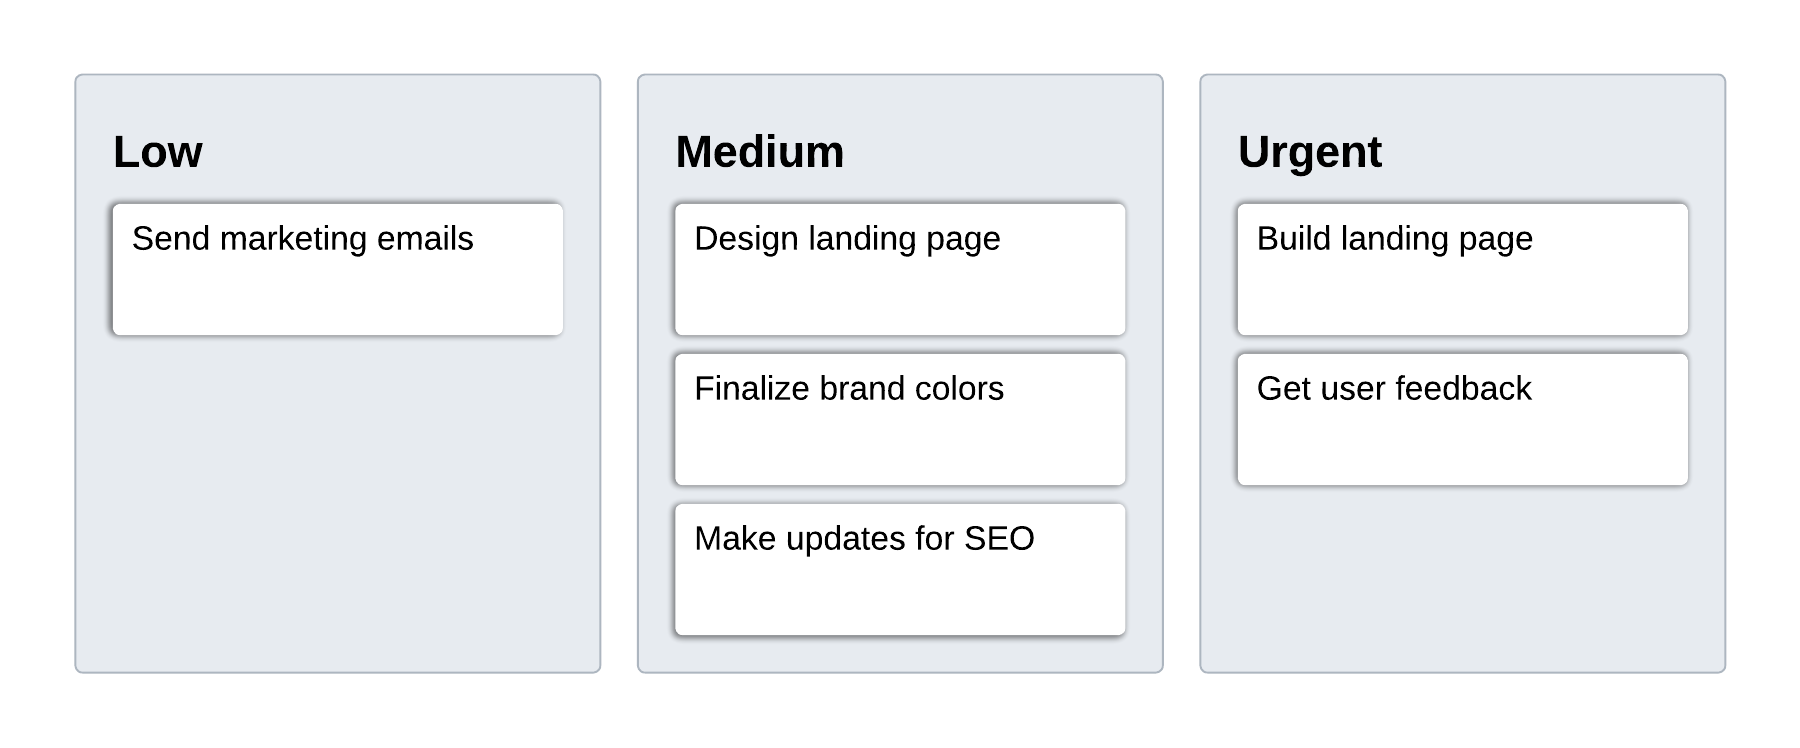
\includegraphics[width=0.8\textwidth]{diagrams/ebql-architecture.png}
    \caption{The eBQL system architecture. eBQL transforms an extended-SQL query into an abstract
    syntax tree, analyzes the query, then generating an eBPF program to execute the query. The
    program is then loaded into the kernel, and post-processed HFT data is streamed to the user.}
    \label{fig:ebql-architecture}
\end{figure}
eBQL transforms high-level extended-SQL queries through a series of steps before generating an eBPF
tracing program, loading it into the kernel, and streaming output results to the user (Figure
\ref{fig:ebql-architecture}). Crucially, the internals of eBPF is abstracted away from the user,
enabling HFT data collection in a declarative manner.

\subsection{eBQL API}
\label{ebql-api}

From a client perspective, eBQL exposes a simple query executor API with just two methods beyond a
default initialization: % (Figure \ref{code:ebql-api}).

% \begin{figure}[htpb]
\begin{lstlisting}
pub struct Executor {
    /// internal fields
}

impl Executor {
    /// Initializes an empty query executor.
    pub fn new() -> Executor;

    /// Executes an extended-SQL query.
    pub fn execute_query(
        &mut self,
        sql_query: String,
    ) -> Result<(Arc<Schema>, Receiver<RecordBatch>)>;

    /// Fetches the stats of a specific query.
    pub fn get_query_stats(&self, q: String) -> Option<QueryStats>;
}
\end{lstlisting}
% \caption{The eBQL API.}
% \label{code:ebql-api}
% \end{figure}

After initializing with \texttt{Executor::new()}, the executor takes in an extended-SQL query
(\S \ref{query-language}) and converts it into an eBPF instrumentation program executing in the
kernel. If successful, the executor returns the query's schema definition (\S 
\ref{data-rep-out}), and a receiver channel of streamed record batches (i.e., HFT data after being
processed by the query).


\subsection{Query Language}
\label{query-language}

To enable declarative querying, eBQL exposes a query language lightly extended from SQL.

At its core, eBQL supports the standard SQL functionality, using its relational operator set to
express typical data manipulation. However, eBQL extends standard SQL to support streaming semantics
using a \texttt{Window} operator, and adds additional support for time-series analysis via
histograms and quantiles (Table \ref{tab:ebql-ops} provides a complete operator list). In addition,
eBQL expands SQL’s syntax slightly to accommodate for the kernel event format.

\begin{table}[htpb]
    \centering
    \caption{Operators used in eBQL query plans.}
    \label{tab:ebql-ops}
    \begin{tabular}{|l|p{0.8\linewidth}|}
        \hline
        \multicolumn{1}{|c|}{\textit{\textbf{Operator}}} &
        \multicolumn{1}{c|}{\textit{\textbf{Description}}}
        \tabularnewline \hline
        Select & Selects a stream from a kernel tracing event, such as
        \texttt{tracepoint/filemap/mm\_filemap\_add\_to\_page\_cache}. \\
        \hline
        Window & Partitions unbounded streams into bounded relations, either by \texttt{time} or
        tuple \texttt{count}. Windows have a \texttt{step} value (either some time interval or
        tuple amount) $\le $ the window size.\\
        \hline
        Project & Selects specific attributes from a stream/relation. These attributes may be
        event-specific (e.g. \texttt{pfn} for page cache evictions), or generic system attributes
        (e.g. \texttt{pid/tgid}, \texttt{cgroup}, or CPU/SMP id).\\
        \hline
        Filter & Filters attributes based on some conditional statement, such as \texttt{pid ==
        12000}, or \texttt{count >= 4096}. \\
        \hline
        Map & Maps attributes from one value to another. Example maps use basic arithmetic (e.g.
        \texttt{count * 2}) or available BPF helper functions (e.g.
        \texttt{bpf\_get\_ns\_current\_pid\_tgid(dev, ino)}). \\
        \hline
        GroupBy & Groups events according to a set of grouping keys (e.g. \texttt{(fd, cpu)}).\\
        \hline
        Aggregate & Performs some aggregation over grouped elements. Supported aggregations are
        \texttt{max}, \texttt{min}, \texttt{sum}, \texttt{average}, \texttt{count},
        (linear/exponential) \texttt{histogram}s, and \texttt{quantile}s. \\
        \hline
        Distinct & Eliminates duplicates according to the group by key, preserving the most recent
        event. \\
        \hline
        Join & Joins two event streams by some specified condition (e.g. \texttt{A.pid == B.pid}).\\
        \hline
    \end{tabular}
\end{table}

The design of eBQL's query language is heavily inspired by the Continuous Query Language (CQL) from
Stanford's Data Stream Management System (ref: STREAM, CQL).

The kernel event is initially represented as a \textit{stream} ordered by some time domain (in this
context, the \texttt{ktime == clock\_gettime(CLOCK\_MONOTONIC)}). The \texttt{Window} operator can
then convert the kernel event stream into a bounded \textit{relation} by providing a sliding window
over the stream. eBQL's operators can operate on streams and/or relations, depending on their type:
\begin{itemize}
    \item Stateless operators like project, filter, and map can operate on either streams or
        relations, as each operates only on individual events and thus do not require some bounded
        amount of events to compute.
    \item Ungrouped stateful aggregations can operate on streams, accumulating values until the
        query is finished. This is permitted due to the minimal amount of state needed to store
        aggregation values: for instance, a \textit{count} aggregation without grouping requires
        only a constant amount of space---one \texttt{u64}---regardless of the amount of elements in
        the stream.
    \item Stateful (grouped) aggregations can also operate on bounded (i.e. windowed) relations.
        Data manipulation with these constructs perform the same functionality as their standard SQL
        equivalents: for instance, the \texttt{max} computed over a $1024$-count window is
        functionally equivalent to a \texttt{max} computed over a $1024$-row relation.
    \item Joins can only operate on relations: they must compute the result on the entire input
        before results are produced, so the input sources must be bounded relations, not unbounded
        streams.
\end{itemize}

From a user standpoint, besides from the additional \texttt{Window} operator to accommodate the
streaming nature of kernel events, eBQL's query language models the same semantics as standard SQL
with only slight syntactical differences.

As an example, Figure \ref{code:ebql-ex} shows a continuous aggregation query over \texttt{pread64}
syscall invocations.
\begin{figure}[htpb]
\begin{lstlisting}[language=SQL]
SELECT fd, cpu, COUNT(*), MAX(count), AVG(count)
    FROM tracepoint/syscalls/sys_enter_pread64
    GROUP BY fd, cpu
    WHERE pid == 1041370
    WINDOW(time, 1000, 1000);
\end{lstlisting}
\caption{A continuous eBQL aggregation query. The additional \texttt{Window} operator converts the
event stream into a relation: the first argument takes in the window type (\texttt{time} or
\texttt{count}), the second argument the interval, and the third argument the step size (for time,
in milliseconds).}
\label{code:ebql-ex}
\end{figure}

The query establishes a tumbling 1 second \texttt{time} window over the \texttt{sys\_enter\_pread64}
tracepoint, filters for syscalls from only the specified \texttt{pid} (here \texttt{1041370}), then
groups all invocations on the same \texttt{fd} and from the same \texttt{cpu}, and computes three
aggregations: the total number of elements, the maximum number of bytes read, and the average amount
of bytes read (for context, \texttt{count} in the \texttt{pread64} syscall represents the amount of
bytes to read).

The query then returns events every time the window steps forward (here, every second) as a
\texttt{RecordBatch} (Section \ref{data-rep-out}).

\subsection{Data Representation}
\label{data-rep}

\subsubsection{Relational Model}
Within eBQL, each kernel event is modeled as a \textit{streaming relation} with a fixed set of
attributes.

The existing kernel infrastructure inherently exposes a relational structure for its tracing events:
all (raw) tracepoints follow a fixed format (in Linux, defined at
\texttt{/sys/kernel/tracing /events/<category>/<name>/<format>}), while u[ret]probes and k[ret]probes
expose some probe-specific context with a general fixed structure. Thus, overlaying a relational
structure on top of kernel events provides almost a direct mapping from internal kernel
representations.

Selecting from a kernel event is then semantically equivalent to selecting from a data stream with a
fixed relational definition. For example, the \texttt{sys\_enter\_pread64} tracepoint (with
definition in Figure \ref{code:pread64-format}) is modeled as a relation with four fields,
\texttt{fd}, \texttt{buf}, \texttt{count}, and \texttt{pos} (which are also the arguments to
\texttt{pread64} (ref: pread64 manpage)). 

\begin{figure}[htpb]
\begin{lstlisting}[language=C]
name: sys_enter_pread64
ID: 697
format:
    // Four other fields, prefixed common_<field>, exist, but are not available to eBPF programs attached to tracepoints, and are thus omitted.
    field:int __syscall_nr; offset:8;   size:4; signed:1;
    field:unsigned int fd;  offset:16;  size:8; signed:0;
    field:char * buf;   offset:24;  size:8; signed:0;
    field:size_t count; offset:32;  size:8; signed:0;
    field:loff_t pos;   offset:40;  size:8; signed:0;
\end{lstlisting}
\caption{The \texttt{sys\_enter\_pread64} tracepoint definition, from
\texttt{/sys/kernel/tracing/events/syscalls/sys\_enter\_pread64/format}.}
\label{code:pread64-format}
\end{figure}

However, there are some important caveats to the relational model.

First, an event's context alone does not fully represent the context available. At each event, the
kernel exposes a generic set of system values (included, but not limited to, \texttt{ktime},
\texttt{pid/tgid}, \texttt{cgroup}, \texttt{cpu}, \texttt{comm}, and \texttt{task}).  Thus, in
addition to the event-specific context, each event's relational model additionally exposes a fixed
set of system attributes.

Second, many events contain complicated kernel structures. The system \texttt{task} struct is a
huge, deeply nested, struct; and in \texttt{block} IO tracepoints, the \texttt{request} struct
(Figure \ref{code:request-struct}) contains copious amounts of information, such as the
\texttt{gendisk}, \texttt{block\_device}, and more metadata.  To represent and access this data, the
relation contains a type resembling SQL's \texttt{STRUCT} complex type. 

\begin{figure}[htpb]
\begin{lstlisting}[language=C]
struct request {
    // ... additional fields ...  
    struct gendisk *rq_disk;
    struct block_device *part;
    u64 alloc_time_ns;
    u64 start_time_ns;
    u64 io_start_time_ns;
    short unsigned int wbt_flags;
    short unsigned int stats_sectors;
    // ... additional fields ...  
}
\end{lstlisting}
\caption{The \texttt{struct request} type at \texttt{block} IO tracepoints. Access would then
require nested de-references; for instance, accessing the first minor device number of a block IO
request would be \texttt{request.rq\_disk.first\_minor}.}
\label{code:request-struct}
\end{figure}

Because of these two cases, the event relational model is, in a sense, \textit{denormalized}. Each
relation contains attributes that are not specific to them, but rather available at many relations:
every relation contains generic system attributes, and for similar tracepoints (like the
\texttt{block} IO ones), each context contains ``duplicate'' attribute definitions for identical
structs.

However, this denormalization does not impose additional access or storage overhead. Each event
stream does not literally store all attributes in memory; rather, on every invocation, the BPF
program has \textit{read-only access} to contexts stored in \textit{existing} kernel memory,
requiring no additional storage. For instance, each process already has a \texttt{task} struct
associated with it in the kernel, and \texttt{block} IO requests already require a \texttt{request}
struct to be created somewhere in-kernel.

\subsubsection{Query Output}

Each query projects some subset of a kernel event and optionally performs some
aggregations/transformations on the data. To provide a structured representation, the query output
is represented as a \texttt{RecordBatch}:
\begin{lstlisting}
pub struct RecordBatch {
    pub schema: Arc<Schema>,
    pub records: Vec<Record>,
}
\end{lstlisting}

Each record batch contains the query's output \texttt{Schema} with a fixed set of
\texttt{DataType}s, with a collection of \texttt{Record}s representing the actual
\texttt{DataValue}s of each output record. \texttt{RecordBatch}es are streamed from queries whenever
the window steps forward.

The \texttt{RecordBatch} structure is intentionally modeled after existing database libraries'
representations, like \texttt{sqlx} (ref: sqlx) and Apache Arrow (ref: arrow).

\label{data-rep-out}

\subsection{Query Plans}

Given an extended-SQL query, eBQL then compiles it into a \textit{query plan} that represents the
query procedure. The conceptual query plan is again inspired heavily by CQL's design (ref: CQL).

Each query plan is composed of eBQL operators, similar to SQL query plans. For instance, the query
in Figure \ref{code:ebql-ex} has the following logical plan:

\begin{lstlisting}[language=C]
Select(tracepoint/syscalls/sys_enter_pread64)
    .Window(time, 1000ms, 1000ms)
    .Project(fd, cpu, count, pid, time)
    .Filter(pid == 1041370)
    .GroupBy(fd, cpu)
    .Aggregate(Count)
    .Aggregate(Max, count)
    .Aggregate(Average, count);
\end{lstlisting}

Conceptually, new events flow between operators via \textit{queues} that store intermediate results
between operators, and stateful operators store persistent values in \textit{synopses}. On window
steps, results stored in synopses are emitted, and expired events again flow through operators,
clearing themselves from any synopses that contain their state.

\subsubsection{Physical Plan and Query Optimization}

The physical implementation of a query plan is split into two components, the \textit{kernel-space}
and \textit{user-space} component. A key consideration is determining when to emit to user-space, as
communicating values from kernel-space to user-space incurs substantial overhead.

Specifically, eBPF programs emit values to user-space through a concurrent MPSC ring buffer
implemented as a BPF map (\texttt{BPF\_MAP\_TYPE\_RINGBUF}), which is consumed by a user-space
process. Much work has been done to optimize the data transmission, with memory-mapped pages
available to user-space applications to avoid kernel-to-user copying and support for \texttt{epoll}
or busy polling (ref: linux ringbuf docs). However, the context switching from user to kernel space,
synchronization and locking overhead of the ringbuf, and interrupt request work processing required
for polling, and more incur prohibitive overhead (we later evaluate these claims in
\S\ref{perf-drilldown}).

Thus, eBQL attempts to process records entirely in kernel space, emitting only the final results, as
this reduces the total number of events that must be emitted between kernel to user space. For now,
eBQL's query planning places any operator that can feasibly be implemented within eBPF's constraints
into kernel space, only deferring to user-space when an operator is not possible in kernel space.
Specifically, all operators except for general Joins and non-tumbling time windows are implemented
purely in kernel space (because eBPF does not have dynamic memory or non-constant-bounded loops,
Joins and non-tumbling time windows---which require unbounded loops---cannot currently be
implemented in eBPF).

Beyond the user-kernel space split, eBQL also performs standard logical query optimizations, such as
predicate pushdown, split conjunctive predicates, and projection pushdown (ref: pred pushdown).
Although BPF programs are not querying external storage---and thus materializing records/attributes
and its associated IO cost is not a factor---minimizing attribute materialization still provides
potentially significant performance benefits. This is because BPF programs do not have direct access
to all kernel memory; thus, system attributes require BPF helper functions to access such as
\texttt{bpf\_ktime\_get\_ns}---which can incur non-trivial overhead---and reading certain kernel
memory requires the \texttt{bpf\_probe\_read\_kernel} helper function, incurring significant
overhead due to memory copying and a dependency on variable arguments that requires runtime checks
for safety (ref: ebpf runtime policies, bpf probe read kernel source).

eBQL also takes advantage of the restriction to tumbling windows in eBPF to simplify windowing and
aggregation logic. In tumbling windows, every window step discards every element in the previous
window; thus, windowing needs only to record a constant amount of metadata to determine when to
tumble (e.g. items seen for count-based windows, or the start timestamp for time-based windows), and
every stateful operator simply clears its synopses, an almost-constant time operation (eBPF does not
support clearing maps in kernel-space, so it requires a map iteration to delete each element;
however, when values are grouped, the number of group-by keys is often significantly less than the
total amount of elements).

Currently, eBQL only employs rule-based optimization. However, recent work attempts to quantify the
cost of BPF operations (ref: ebpf runtime policies); thus, future work can explore estimates using
data characteristics to perform cost-based optimizations. For instance, if an eBPF operator requires
a high amount of costly function invocations or redundant memory allocation in BPF maps, it might be
more optimal to incur the kernel-user data transmission overhead and defer computation to user
space.

Operator implementations in user-space follow standard database operator implementations (for
instance, a Join could be implemented as a grace hash join or index nested loop join), and are thus
elided.

\subsection{Code Generation}

After processing the query plan, eBQL converts the kernel-space operators into BPF C code.

\texttt{bpftrace} implements a full fledged AST-LLVM IR-eBPF bytecode transformation pipeline;
however, \texttt{bpftrace} aims to support arbitrary procedural logic (an example is Figure
\ref{code:bpftrace-ex}). Due to the constrained set of operators available in eBQL, it opts for a
simpler approach of composing together multiple operator representations and generating a collection
of output header files, with struct, map, and operator definitions in C, included into one source
file (details can be found in \S\ref{impl-codegen}).

The generated C code is then dispatched to \texttt{clang}, which compiles it down into eBPF
bytecode.

\subsection{Query Execution and Post-Processing}

eBQL then loads the generated eBPF bytecode into the kernel, where the eBPF verifier checks the
query for validity (because eBQL's internal catalog should handle logical bindings, and the codegen
step should properly adhere to eBPF requirements, users are abstracted away from verifier
peculiarities; failure at the verifier indicates a bug in eBQL itself, not in the user query).

eBQL then processes the loaded BPF objects, setting global flags and optionally pinning maps (a
feature useful for synopsis sharing, but not currently implemented by eBQL) before attaching the
program to the kernel event. At this point, the generated BPF program is now running in the kernel,
and query output is streamed to the user.

% \subsection{References}
% \begin{itemize}
    % \item STREAM: data stream management book
    % \item CQL
    % \item sqlx: https://docs.rs/sqlx/0.7.4/sqlx/trait.Database.html\#associatedtype.QueryResult
    % \item apache arrow: https://arrow.apache.org/rust/arrow/record\_batch/struct.RecordBatch.html
    % \item linux ringbuf docs: https://docs.kernel.org/bpf/ringbuf.html
    % \item pred pushdown: https://www.vldb.org/conf/1994/P096.PDF
    % \item bpf runtime policies: https://people.cs.vt.edu/djwillia/papers/ebpf23-runtime.pdf
    % \item bpf probe read kernel source:
        % https://elixir.bootlin.com/linux/v6.7/source/include/linux/bpf.h\#L2742
% \end{itemize}


\section{Implementation}

We implement an eBQL prototype in Rust, with \textasciitilde{}3.5k lines of Rust and
\textasciitilde{}1k lines of C. eBQL is compiled as a Rust library, allowing clients to link into
its API (defined in Section \ref{ebql-api}).

\subsection{eBQL Query Parsing}

To support parsing of eBQL's extended SQL syntax, we extend an existing Rust SQL parser,
\texttt{nom-sql}, which is based on the \texttt{nom} parser combinator framework (ref: nom-sql,
nom). We preferred \texttt{nom-sql} over other SQL parsing libraries like \texttt{sqlparser} (ref:
sqlparser), a top-down operator-precedence (TDOP) parser, due to parser generator frameworks'
general ease of extensibility (and also my personal interest).

We extend \texttt{nom-sql} with support for kernel event syntax (in standard SQL,
slashes---\texttt{/}---are not supported), and eBQL-specific operators, such as \texttt{Window},
\texttt{Histogram}, and \texttt{Quantile}, to support streaming semantics and additional analytics.

\subsection{Code Generation}
\label{impl-codegen}

Stateless operators are relatively straightforward to generate (for instance, an \texttt{Equal(a,
b)} filter becomes \texttt{if (a == b) \{ ... \}}) from the logical plan. Since the BPF stack size
is limited to 512 bytes, eBQL attempts to consolidate projects, filters, and maps and avoid storing
intermediate state on the stack.

Fully generating stateful operators like aggregations and their associated synopses can become
involved; further, the eBPF verifier requires argument types, map definitions, and function
invocations to be statically declared, preventing useful generic programming techniques in C, such
as function parameters and using \texttt{void *}. Thus, codegen is simplified by representing each
stateful operator as a composable \textit{template}; when a specific query plan is compiled into
eBPF code, the template is rendered with the actual values (in some senses, this is similar to
monomorphization; the templates represent the generic parameters, while the rendered code is the
unique instantiation).

Figure \ref{code:agg-tmpl} shows an example template for a \texttt{bpf\_for\_each\_map\_elem}
callback that fetches aggregation values. eBQL uses the Handlebars engine (ref: handlebars) to
render templates into unique instantiations.

\begin{figure}[htpb]
\begin{lstlisting}[language=C]
static __always_inline s64 __get_{{agg}}_{{field_name}}_{{query_name}}_callback(
            struct bpf_map *map,
            group_by_{{query_name}}_t *key,
            agg_t *agg,
            {{agg}}_{{field_name}}_{{query_name}}_ctx_t *ctx) {
    // Skip if aggregation value is 0; this means the value was cleared
    if (agg->val == 0) {
        return 0;
    }
    // Set agg value
    if (!ctx || !ctx->buf) {
        ERROR("Passed null context/context buffer in");
        return 1;
    }
    if (ctx->count >= ctx->buf_sz) {
        WARN("Number of aggregation results exceeds buf size; stopping...");
        return 1;
    }
    {{#each group_bys}}
    ctx->buf[ctx->count].{{field_name}} = key->{{field_name}};
    {{/each}}
    ctx->buf[ctx->count].{{agg}}_{{field_name}} = agg->val;
    ctx->count += 1;
    return 0;
}
\end{lstlisting}
\caption{A template for a callback to retrieve aggregated values using
\texttt{bpf\_for\_each\_map\_elem}.}
\label{code:agg-tmpl}
\end{figure}

Using these templates, the internal stateful operator implementations can be exposed via a single
helper function; thus, in the actual eBPF program code, only that helper function needs to be
invoked, greatly simplifying the codegen into a sequence of operators. A generated eBPF program for
the program in Figure \ref{code:ebql-ex} might then look like this:

\begin{lstlisting}[language=C]
SEC("tp/syscalls/sys_enter_pread64")
u32 pread_query(struct trace_event_raw_sys_enter* ctx) {
    u64 pid = PID();
    if (pid == 1041370) {
        return 1;
    }
    u64 time = TIME();
    u64 fd = ctx->args[0];
    u64 cpu = CPU();
    u64 count = ctx->args[2];
    bool tumble = window_add(time);
    if (tumble) {
        // window tumbling and emitting to user-space logic...
    }
    insert_count__pread_query({fd, cpu}, 1);
    insert_max_count_pread_query({fd, cpu}, count);
    insert_avg_count_pread_query({fd, cpu}, count);
    return 0;
}
\end{lstlisting}

\subsection{Prototype Limitations}

Being a prototype, eBQL has many limitations.

eBQL's query plan analysis is limited, restricting the complexity of generated queries; in
particular, nested aggregations, histograms/quantiles, nested selects, post-aggregation processing,
and joins are not currently supported. Part of this is by design: due to its context of executing in
resource-constrained, performance-sensitive environments, in-kernel queries should incur minimal
overhead and avoid unpredictable runtimes that could spike tail latencies (for instance, a large
binary join every second could skyrocket p99s). Part of it is from verifier restrictions: without
support for dynamic memory or unbounded loops, programs must pre-allocate potentially wasteful
amounts of memory, or are not feasibly implementable (i.e. joins and arbitrary windows).

Part of its limitations is simply due to the code generation step; the method is rather simple,
and does not handle more complicated ASTs yet. Thus, while templated operators enable ease of code
generation, complicated control flow amounts to manual checks and implementation. In the future, it
would be worth exploring potentially harnessing LLVM IR directly (as \texttt{bpftrace} does) to
generate eBPF code, or implementing a more sophisticated compiler.

eBQL currently only supports queries that are feasibly implementable in kernel space; queries that
require complex post-processing in user-space are not supported.


% references:
% \begin{itemize}
    % \item nom-sql, nom
    % \item sqlparser
    % \item handlebars
% \end{itemize}


\section{Evaluation}

Our evaluation seeks to answer the following questions:
\begin{enumerate}
    \item What is the abstraction overhead of eBQL? Do eBQL-generated queries have comparable
        performance to hand-optimized queries? (\S \ref{opt-eval})
    \item How do eBQL-generated queries compare to standard baseline eBPF programs? (\S
        \ref{baseline-eval})
    \item What is the actual overhead of the BPF subsystem, and what benefit does computation
        pushdown into the kernel have? (\S \ref{perf-drilldown})
\end{enumerate}

All evaluations run on a server machine with two Xeon Gold 6150 CPUs (36$\times $ 2.7 GHz) and 377
GiB of RAM. Persistent storage is provided by a Samsung 1TB NVM Drive. The systems runs Ubuntu 22.04
with Linux v5.15.

We evaluate eBQL and hand-written queries using a workload derived from real-world observability
use-cases. Specifically, a \textbf{RocksDB application} under high load continually executes
\texttt{get} commands, reading results from persistent storage. The RocksDB application runs $8$
writer threads concurrently, stopping once 50 million operations are completed.  RocksDB application
randomly selects from pre-generated set of $1,000,000$ keys, each containing a data value of 128
bytes, minimizing the effects of caching. A separate process attaches the eBPF program into the
kernel at the \texttt{sys\_enter\_pread64} tracepoint and collects and processes the outputted data.

Both applications are pinned to a fixed set of 12 CPUs using \texttt{taskset}, carefully chosen to
avoid interference from CPU hyperthreading (we briefly discuss the effect of restricting the number
of cores to 8, such that the RocksDB application then runs within a resource-constrained
environment, with worker threads having competing processes).

Before each benchmark, we run the RocksDB operation individually to reduce any disk caching effects.

\subsection{End-to-End Evaluation}
\label{opt-eval}

We first measure the performance of a query from an eBQL-generated eBPF program compared to a
hand-optimized eBPF program. Ideally, the abstraction overhead of eBQL's higher-level interface and
subsequent query processing steps should be minimal, and provide comparable performance to
hand-optimized programs with a fraction of the developer overhead.

We measure the read throughput achieved by RocksDB, first without any eBPF probes attached to
determine the baseline expected throughput, then with the eBQL-generated eBPF program and the
hand-optimized eBPF program. We also measure a wide range of read latency quantiles to evaluate if
either probe has a significant effect on tail latencies.

Figure \ref{fig:opt-eval-throughput} shows the RocksDB read throughput over the three measurements,
and figure \ref{fig:opt-eval-quantiles} shows the RocksDB read latencies across various quantiles.

\begin{figure}[htpb]
    \centering
    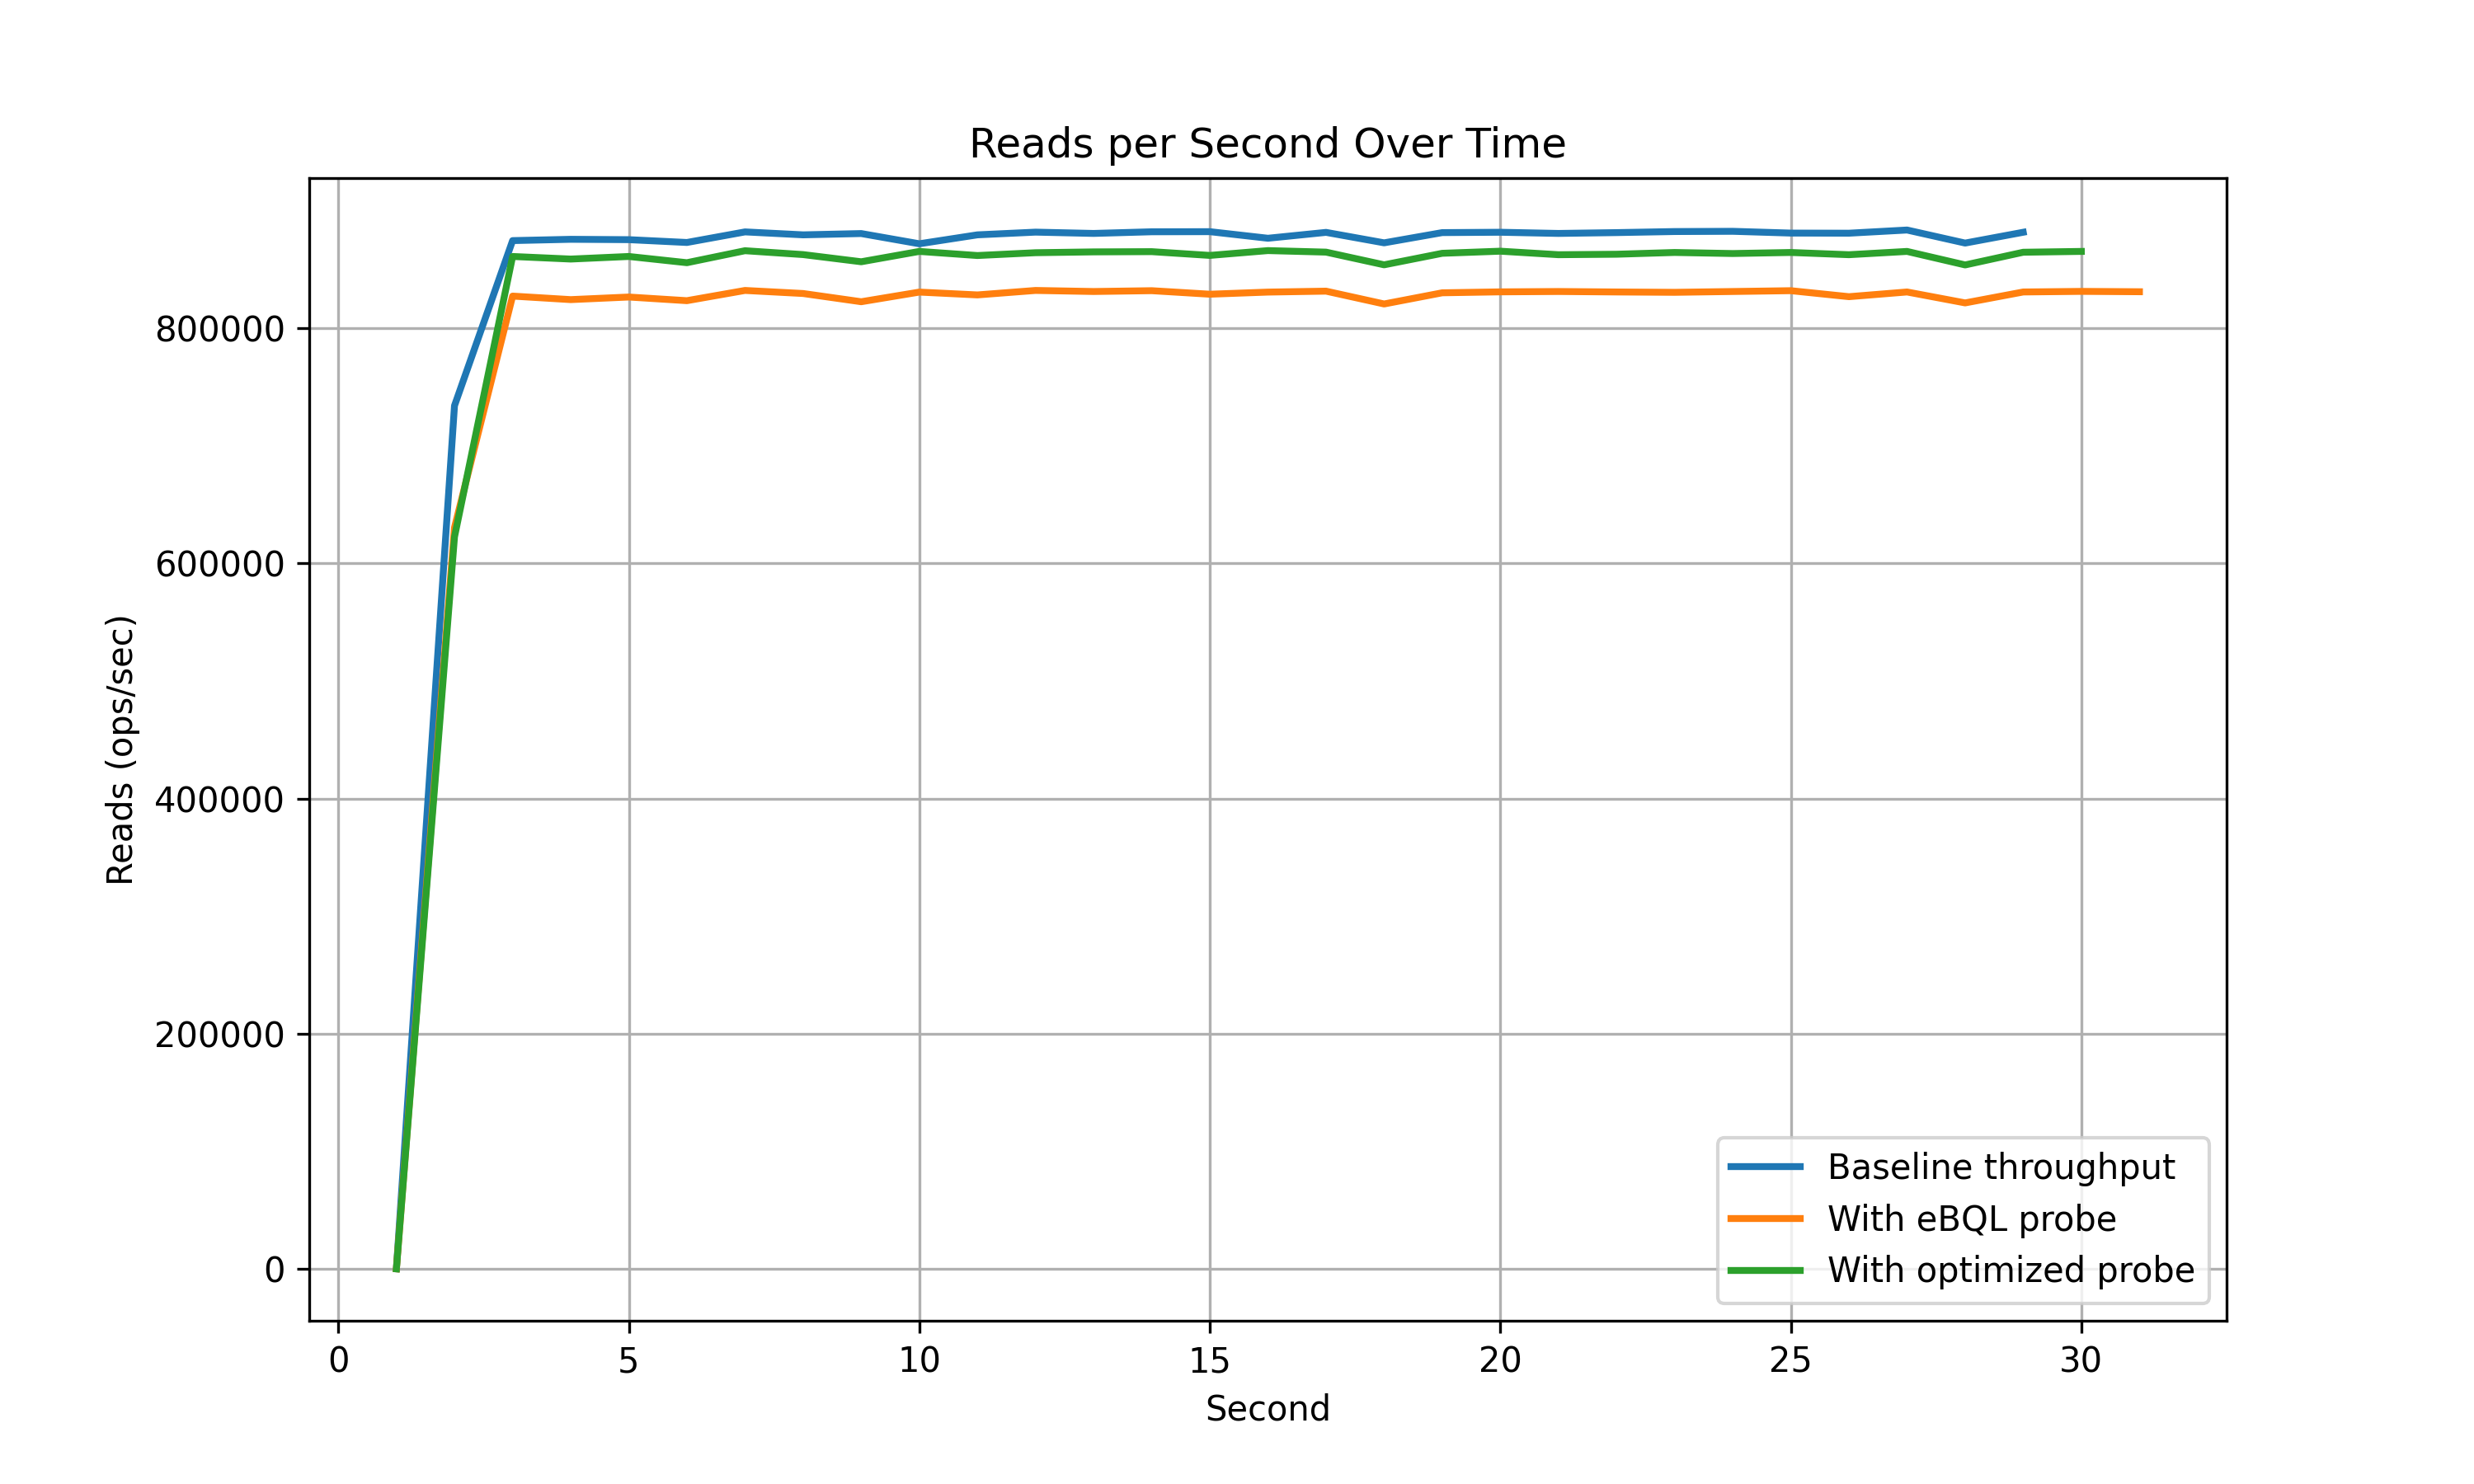
\includegraphics[width=0.6\textwidth]{diagrams/opt-eval-throughput.png}
    \caption{Throughput comparisons between baseline RocksDB without eBPF probes, with an
    eBQL-generated probe, and with a hand-optimized probe.}
    \label{fig:opt-eval-throughput}
\end{figure}

Using 8 worker threads across 12 CPUs, RocksDB achieves a baseline read throughput of $\sim 852k$
operations/second without any probes attached. Once the eBPF probe is attached, the read throughput
drops to $\sim 825k$ operations/second. Using the optimized probe, the read throughput is maintained
at $\sim 838k$ operations/second. Equivalently, the eBQL-generated probe incurs a $3.2\%$ overhead
on reads, compared to the hand-optimized probe's $1.7\%$ overhead.

\begin{figure}[htpb]
    \centering
    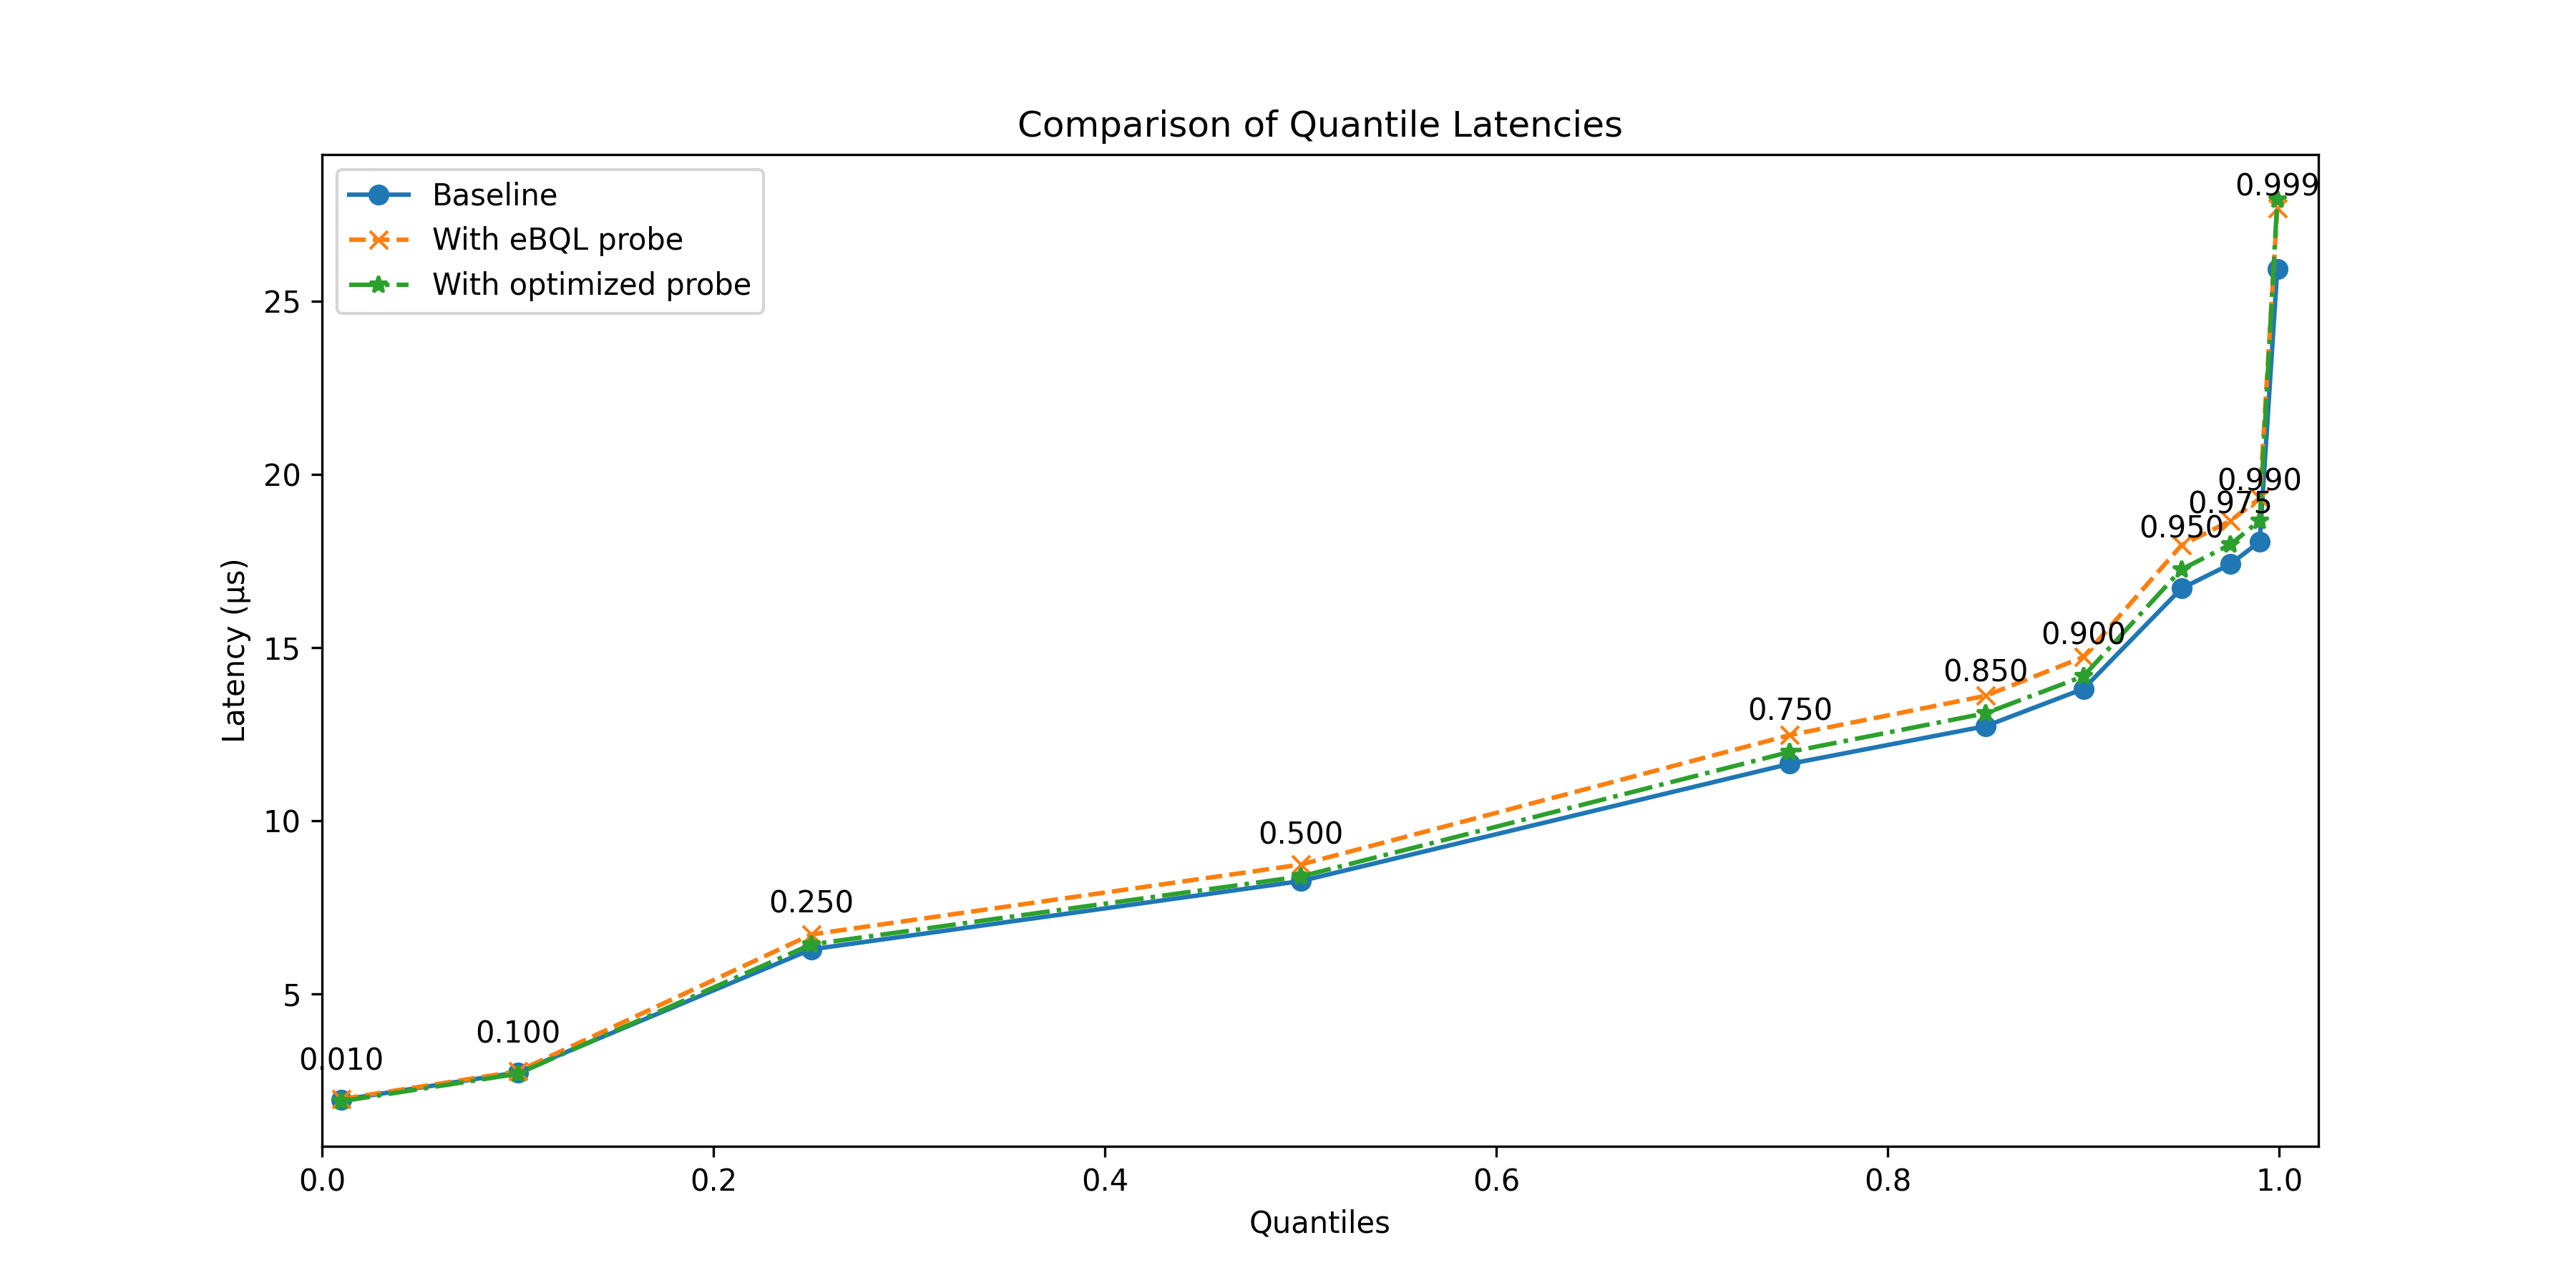
\includegraphics[width=0.8\textwidth]{diagrams/opt-eval-quantiles.png}
    \caption{Quantile comparisons between baseline RocksDB without eBPF probes, with an
    eBQL-generated probe, and with a hand-optimized probe.}
    \label{fig:opt-eval-quantiles}
\end{figure}

A similar result is seen in the quantile measurements: on average ($50\%$ quantile), the baseline
RocksDB read latency without an eBPF probe is $8.338\mu$s, versus $8.606\mu$s with the eBQL probe
($3.2\%$ overhead) and $8.456\mu$s ($1.4\%$ overhead). Despite deferring aggregation computations
and emitting to user-space until the window tumbles, the tail latency is not drastically affected
with the eBPF probe: at the tail ($99.9\%$ quantile) the baseline RocksDB read latency is
$22.437\mu$s, compared to $23.329\mu$s with the eBQL probe ($4.0\%$ overhead) and $22.969\mu$s with
the hand-optimized probe ($2.3\%$ overhead).

\subsection{Evaluation with Baseline eBPF Programs}
\label{baseline-eval}

We then measure the performance compared to a standard baseline eBPF query implementation using
only basic eBPF functionality, one that would feasibly be implemented as a HFT data collection
program.

We use the program presented in Figure \ref{code:pread64-unopt} as the baseline. Although simple,
the pre-requisites to develop an eBPF program like this is non-trivial, requiring knowledge of
tracepoint format and available contexts, program types, BPF helper functions, BPF maps, and the
ringbuf API (ref: bpf-ringbuf nakryiko); moreover, developers must be aware of the verifier
requirements; omitting the null check (\texttt{!q}) outputs a confusing error message that would
require knowledge of eBPF bytecode to decipher.

Compared to the purely kernel-space processing in the eBQL-generated program, the baseline program
defers all query computation to user-space; specifically, since only the raw record is emitted, the
user-space side must handle max/count/average aggregations, groupings, and windowing. This
complicates performance benchmarking. Raw throughput is no longer a fully accurate indicator of
program overhead: instead of the query functionality directly impacting throughput (as eBPF programs
run in kernel context, on the same process, after a hook point is triggered), the vast majority of
query functionality is handled in a separate process managing the eBPF probe.

Thus, for this benchmark we instead measure total CPU cycles as a function of work executed across
both the RocksDB application and the process managing the eBPF probe. This way, the additional query
work is accounted for, even if it did not directly affect throughput. For a direct conversion, on
our machine 100 CPU cycles is 1 second; this value can be determined with
\texttt{sysconf(\_SC\_CLK\_TCK)}. For this, we use \texttt{/proc/<pid>/stat} from \texttt{procfs}
for process cycles, and the BPF subsystem itself for BPF program cycles (via
\texttt{/proc/sys/kernel/bpf\_stats\_enabled}).

We measure five categories of CPU cycles: RocksDB user mode cycles, RocksDB kernel mode cycles, BPF
probe cycles, BPF management process user cycles, and BPF management process kernel cycles. From
these, we can additionally compute the overhead of the BPF subsystem itself by subtracting the
baseline RocksDB kernel mode cycles (the kernel mode cycles for RocksDB-specific work, like
\texttt{pread64} syscalls) and the BPF probe cycles (the BPF probe processing cycles) from the
RocksDB kernel mode cycles with the eBQL/standard-probe attached. To limit variance, we run each
program $50$ times, then compute the average cycle count among all invocations.

\begin{figure}[htpb]
    \centering
    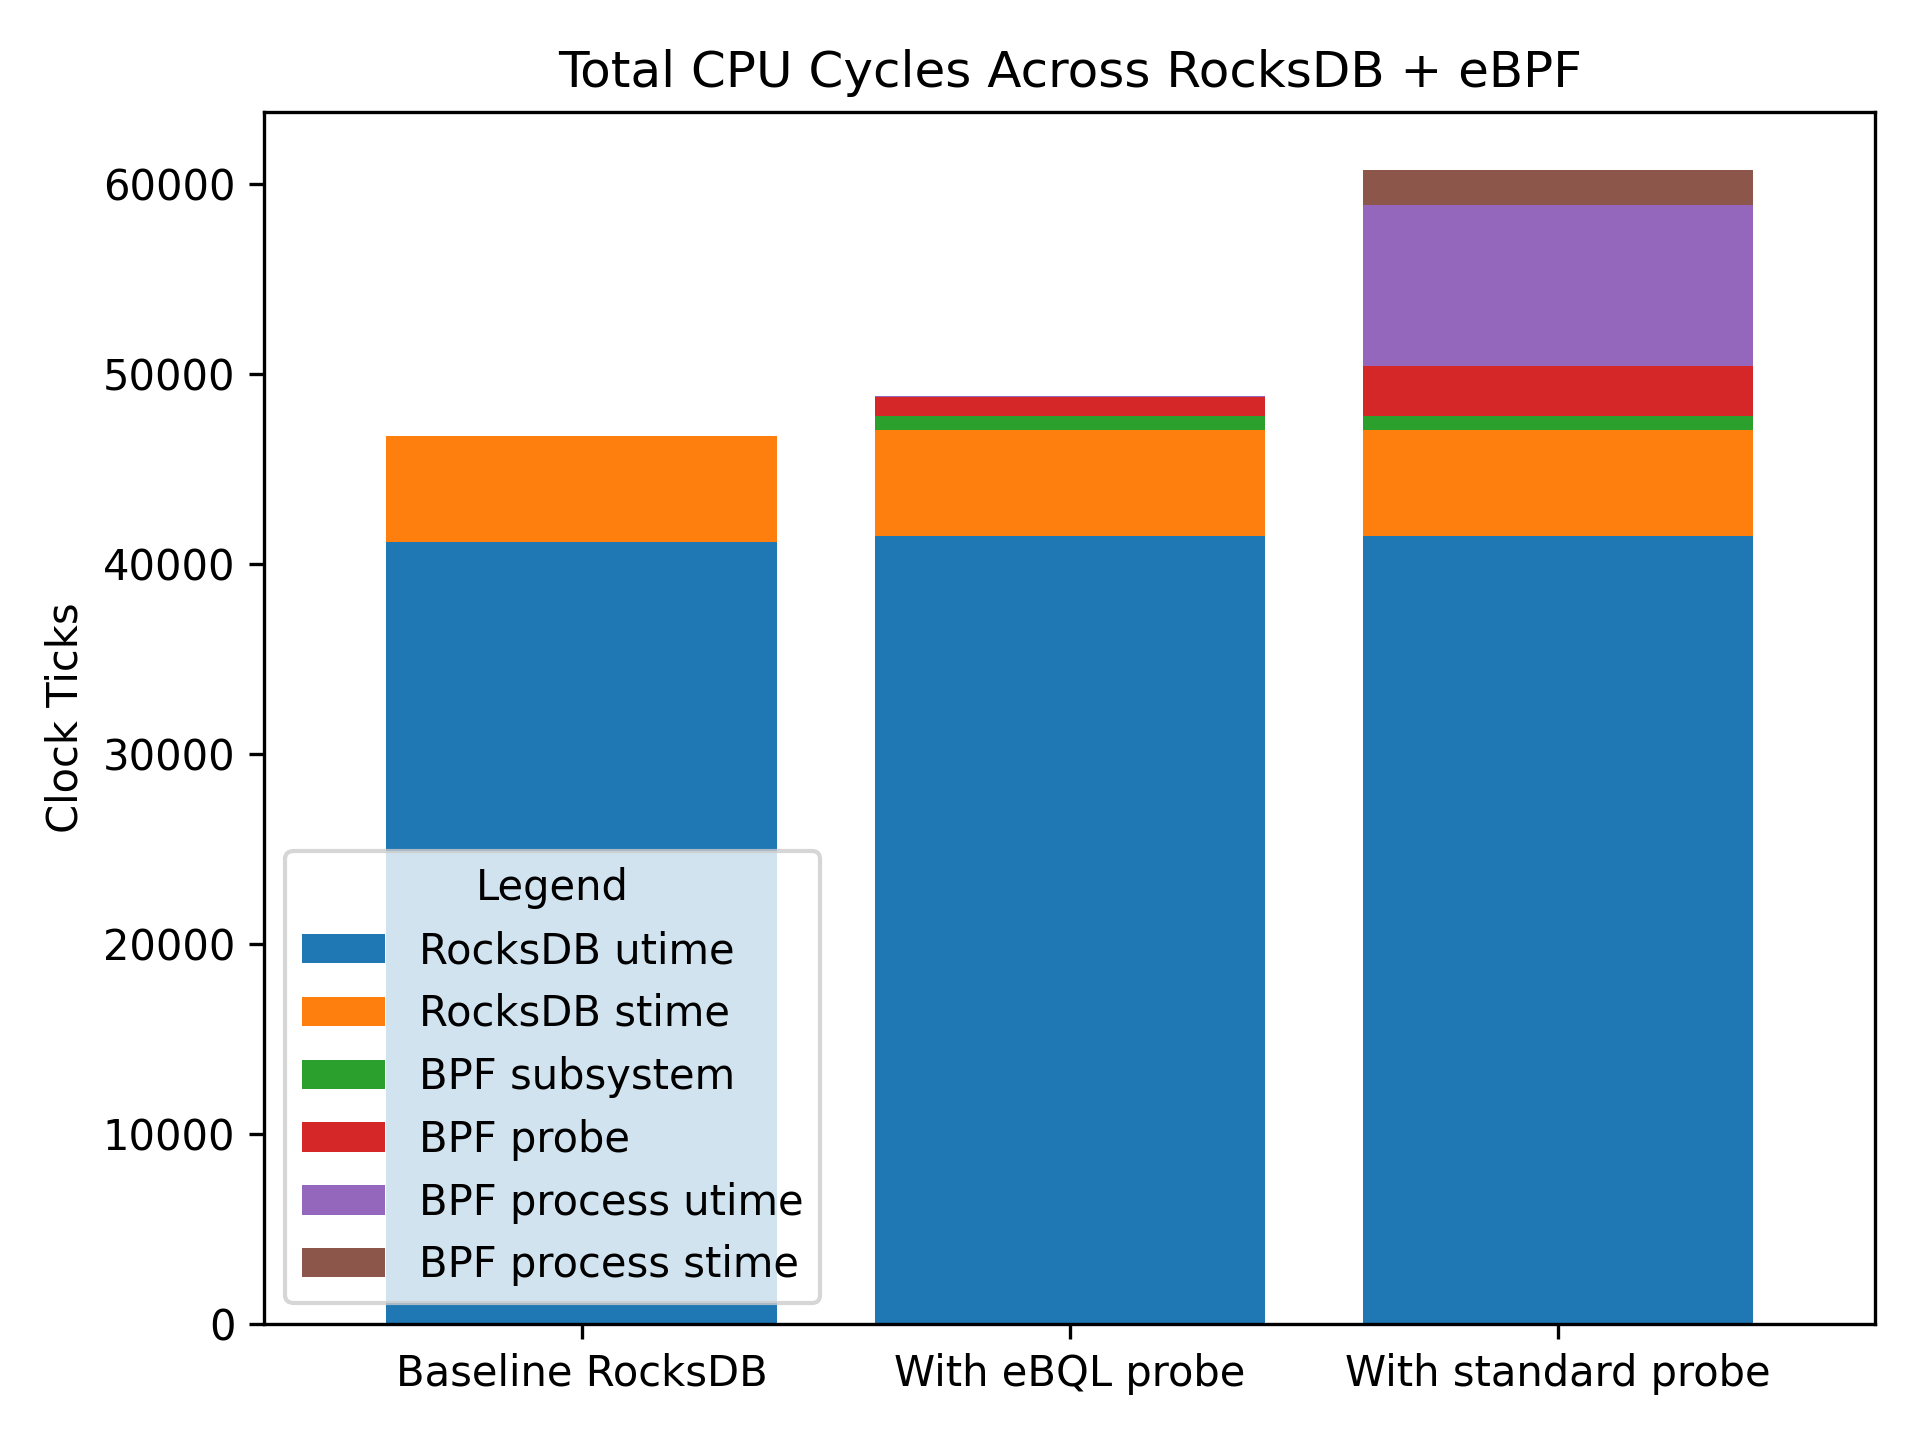
\includegraphics[width=0.6\textwidth]{diagrams/baseline-eval-cycles.png}
    \caption{CPU cycles used between RocksDB without eBPF probes, with an eBQL-generated probe, and
    with a standard probe.}
    \label{fig:baseline-eval-cycles}
\end{figure}

Figure \ref{fig:baseline-eval-cycles} shows the results, and Table \ref{tab:baseline-eval-nums}
contains detailed latency numbers (converted from CPU cycles). Across all programs, the utime/stime
for the RocksDB application itself remained roughly equivalent ($~41450$ cycles). Likewise, the
overhead from the BPF subsystem itself was relatively consistent across programs ($\sim 120$ns per
BPF probe invocation).

\begin{table}[htpb]
    \centering
    \caption{BPF program latencies per run}
    \label{tab:baseline-eval-nums}
    \begin{tabular}{| l | l | l | l |}
        \hline
        \multicolumn{1}{|c|}{\textit{\textbf{Program}}} &
        \multicolumn{1}{c|}{\textit{\textbf{Probe runtime (avg/run)}}} &
        \multicolumn{1}{c|}{\textit{\textbf{BPF subsystem overhead (avg/run)}}} &
        \multicolumn{1}{c|}{\textit{\textbf{Run count}}}
        \tabularnewline \hline
        eBQL & 10.0852s (167.031ns) & 7.587s (125.656ns) & 60379284 \\
        \hline
        Standard & 26.561s (439.708ns) & 7.105s (117.622ns) & 60406223 \\
        \hline
    \end{tabular}
\end{table}

Perhaps surprisingly, despite performing less computation in-kernel, the
standard BPF program actually incurs \textit{more} overhead per BPF probe execution (we investigate
this below, in \S \ref{perf-drilldown}). Further, the managing process must now also devote
significant CPU time towards computing the aggregations in user-space and polling for more data from
kernel-space.

As expected, the standard BPF program consumes more CPU cycles to perform the same query. To further
investigate, we evaluate each probe end-to-end, measuring RocksDB read throughput when both
processes are run on 12 CPUs as before, then on 8 CPUs to simulate a resource-constrained
environment.

Figure \ref{fig:baseline-eval-throughput} shows the results. From the CPU cycles evaluation before,
the 12 CPUs end-to-end evaluation is expected: the eBQL probe outperforms the standard eBPF probe
with less overhead ($3.2\%$ vs $7.2\%$). Further, when constrained to 8 CPUs (and thus the RocksDB
process and the process performing user-space query processing are competing for CPU cycles), the
standard eBPF probe's performance further deteriorates ($17.6\%$ overhead) while the eBQL probe's
performance remains the same.

\begin{figure}
    \centering
    \begin{subfigure}{.5\textwidth}
        \centering
        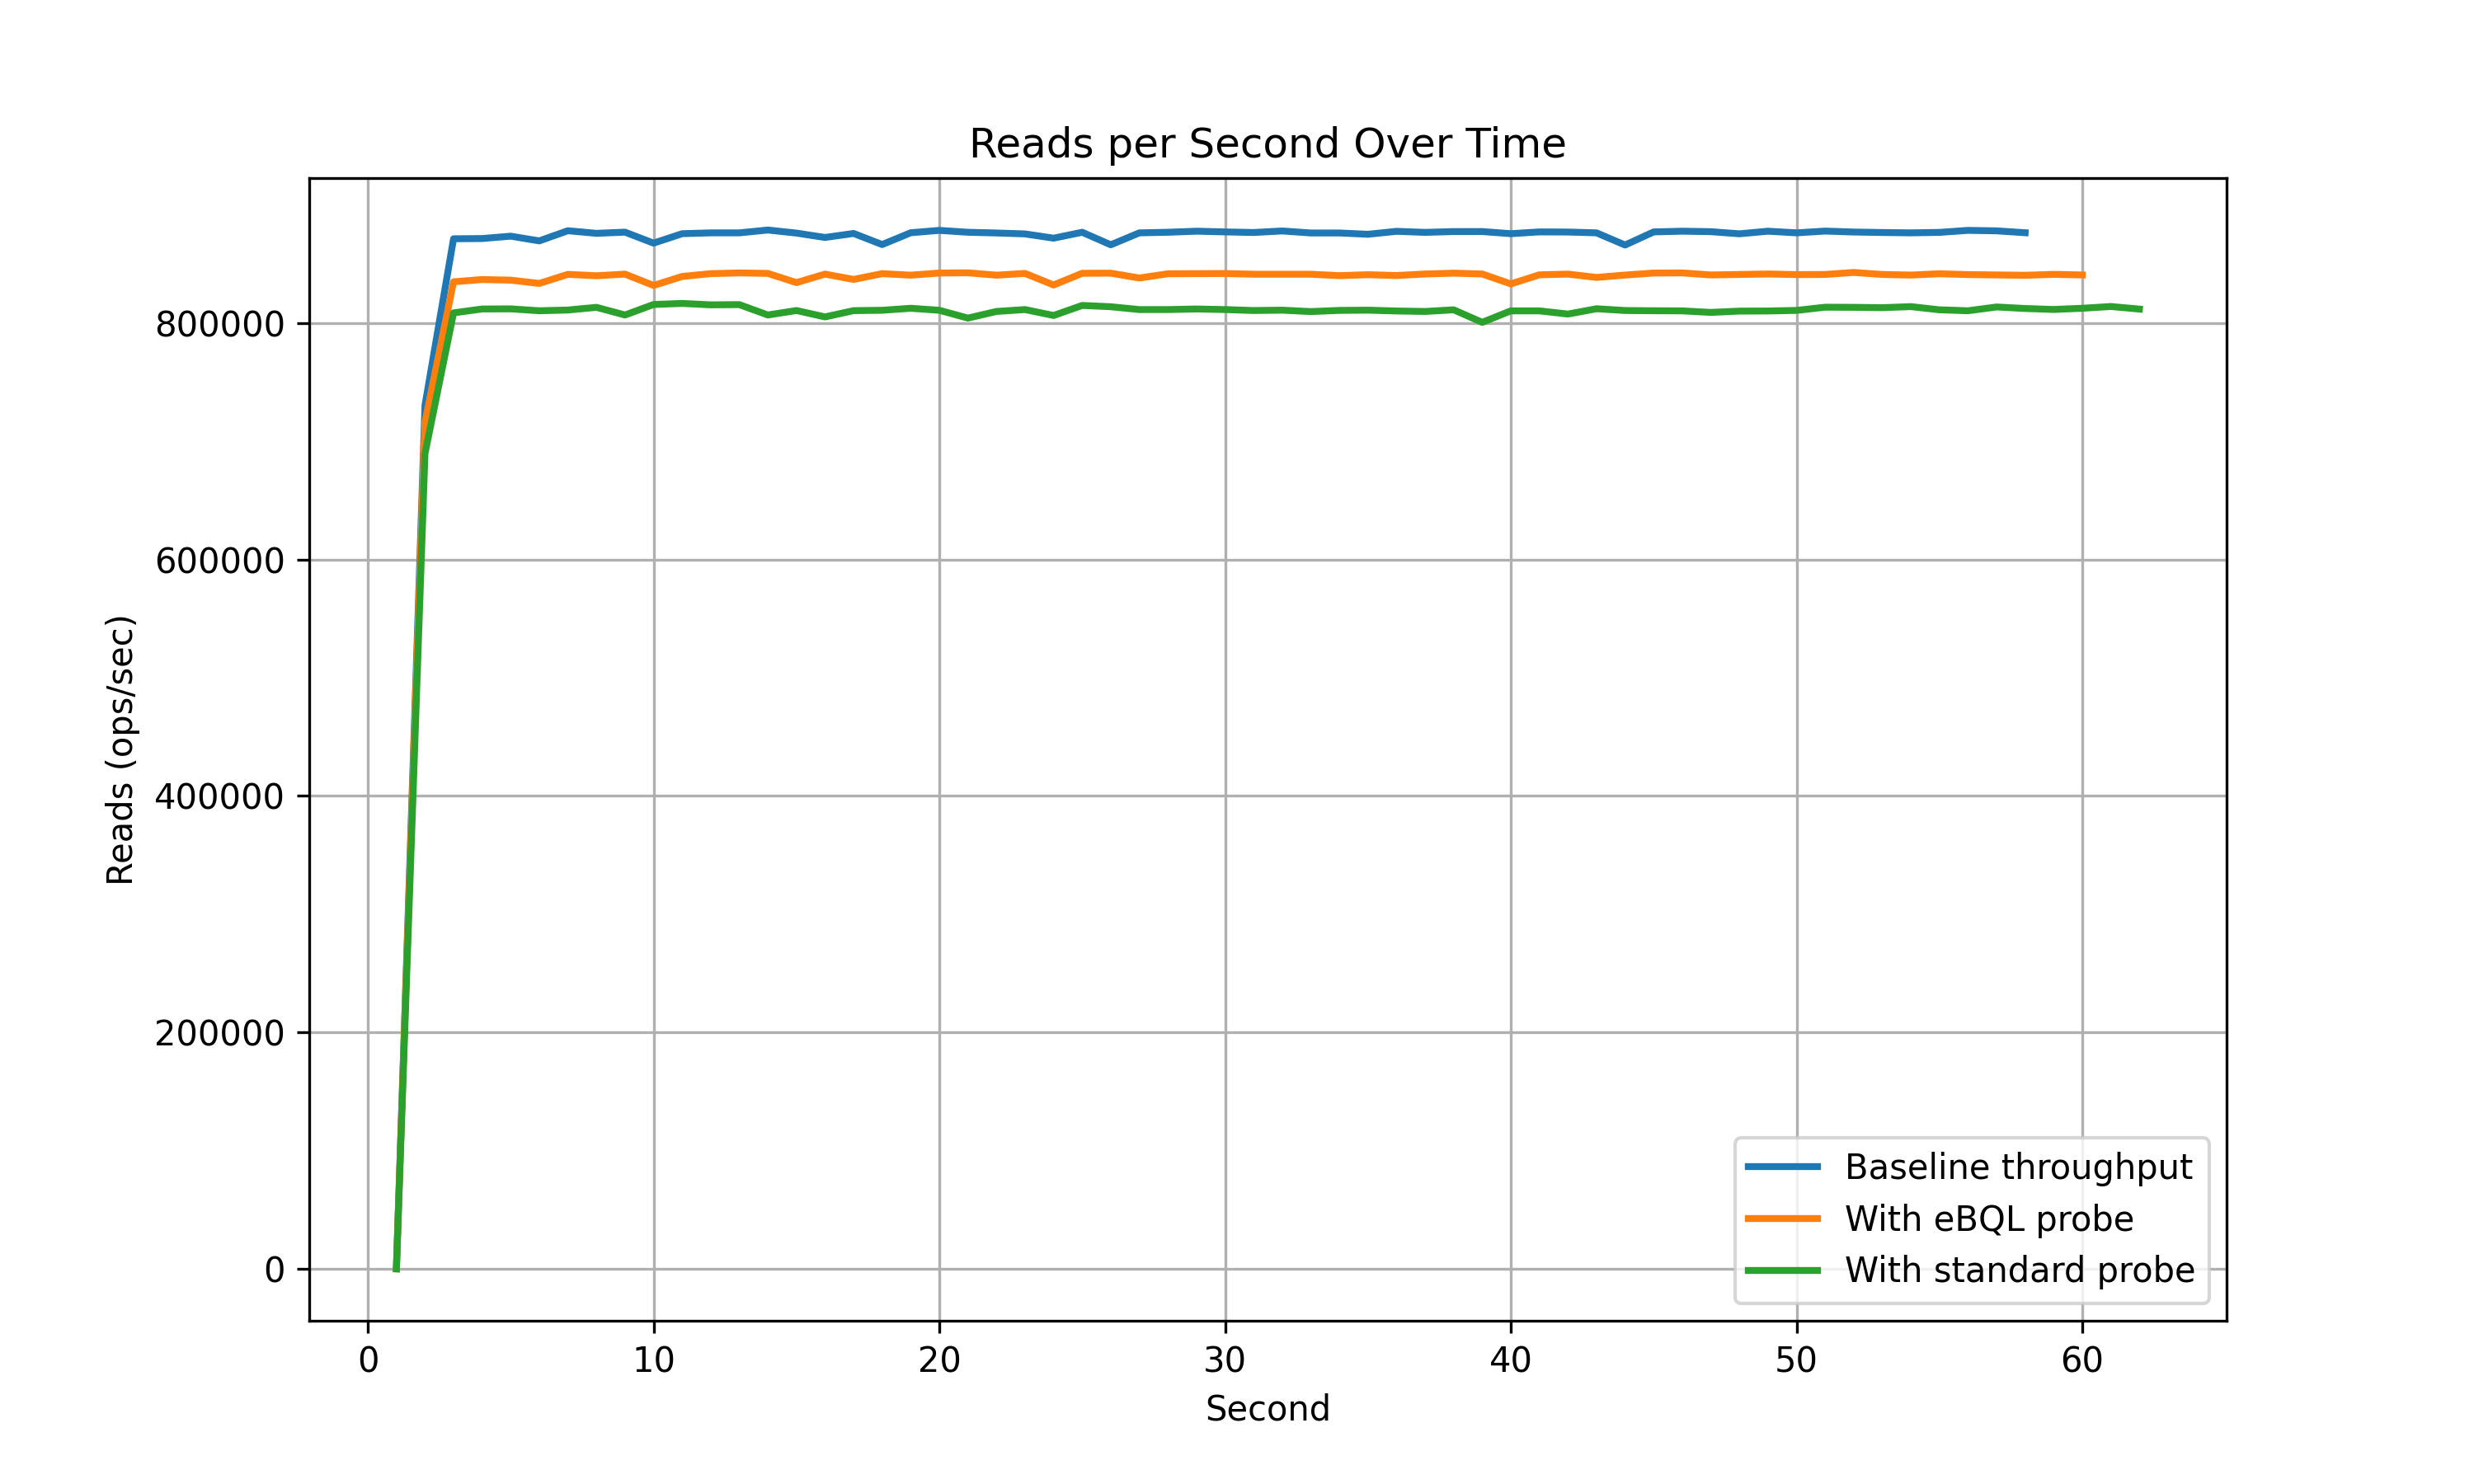
\includegraphics[width=\linewidth]{diagrams/baseline-eval-throughput-12.png}
        \caption{}
        \label{fig:sub1}
    \end{subfigure}%
    \begin{subfigure}{.5\textwidth}
        \centering
        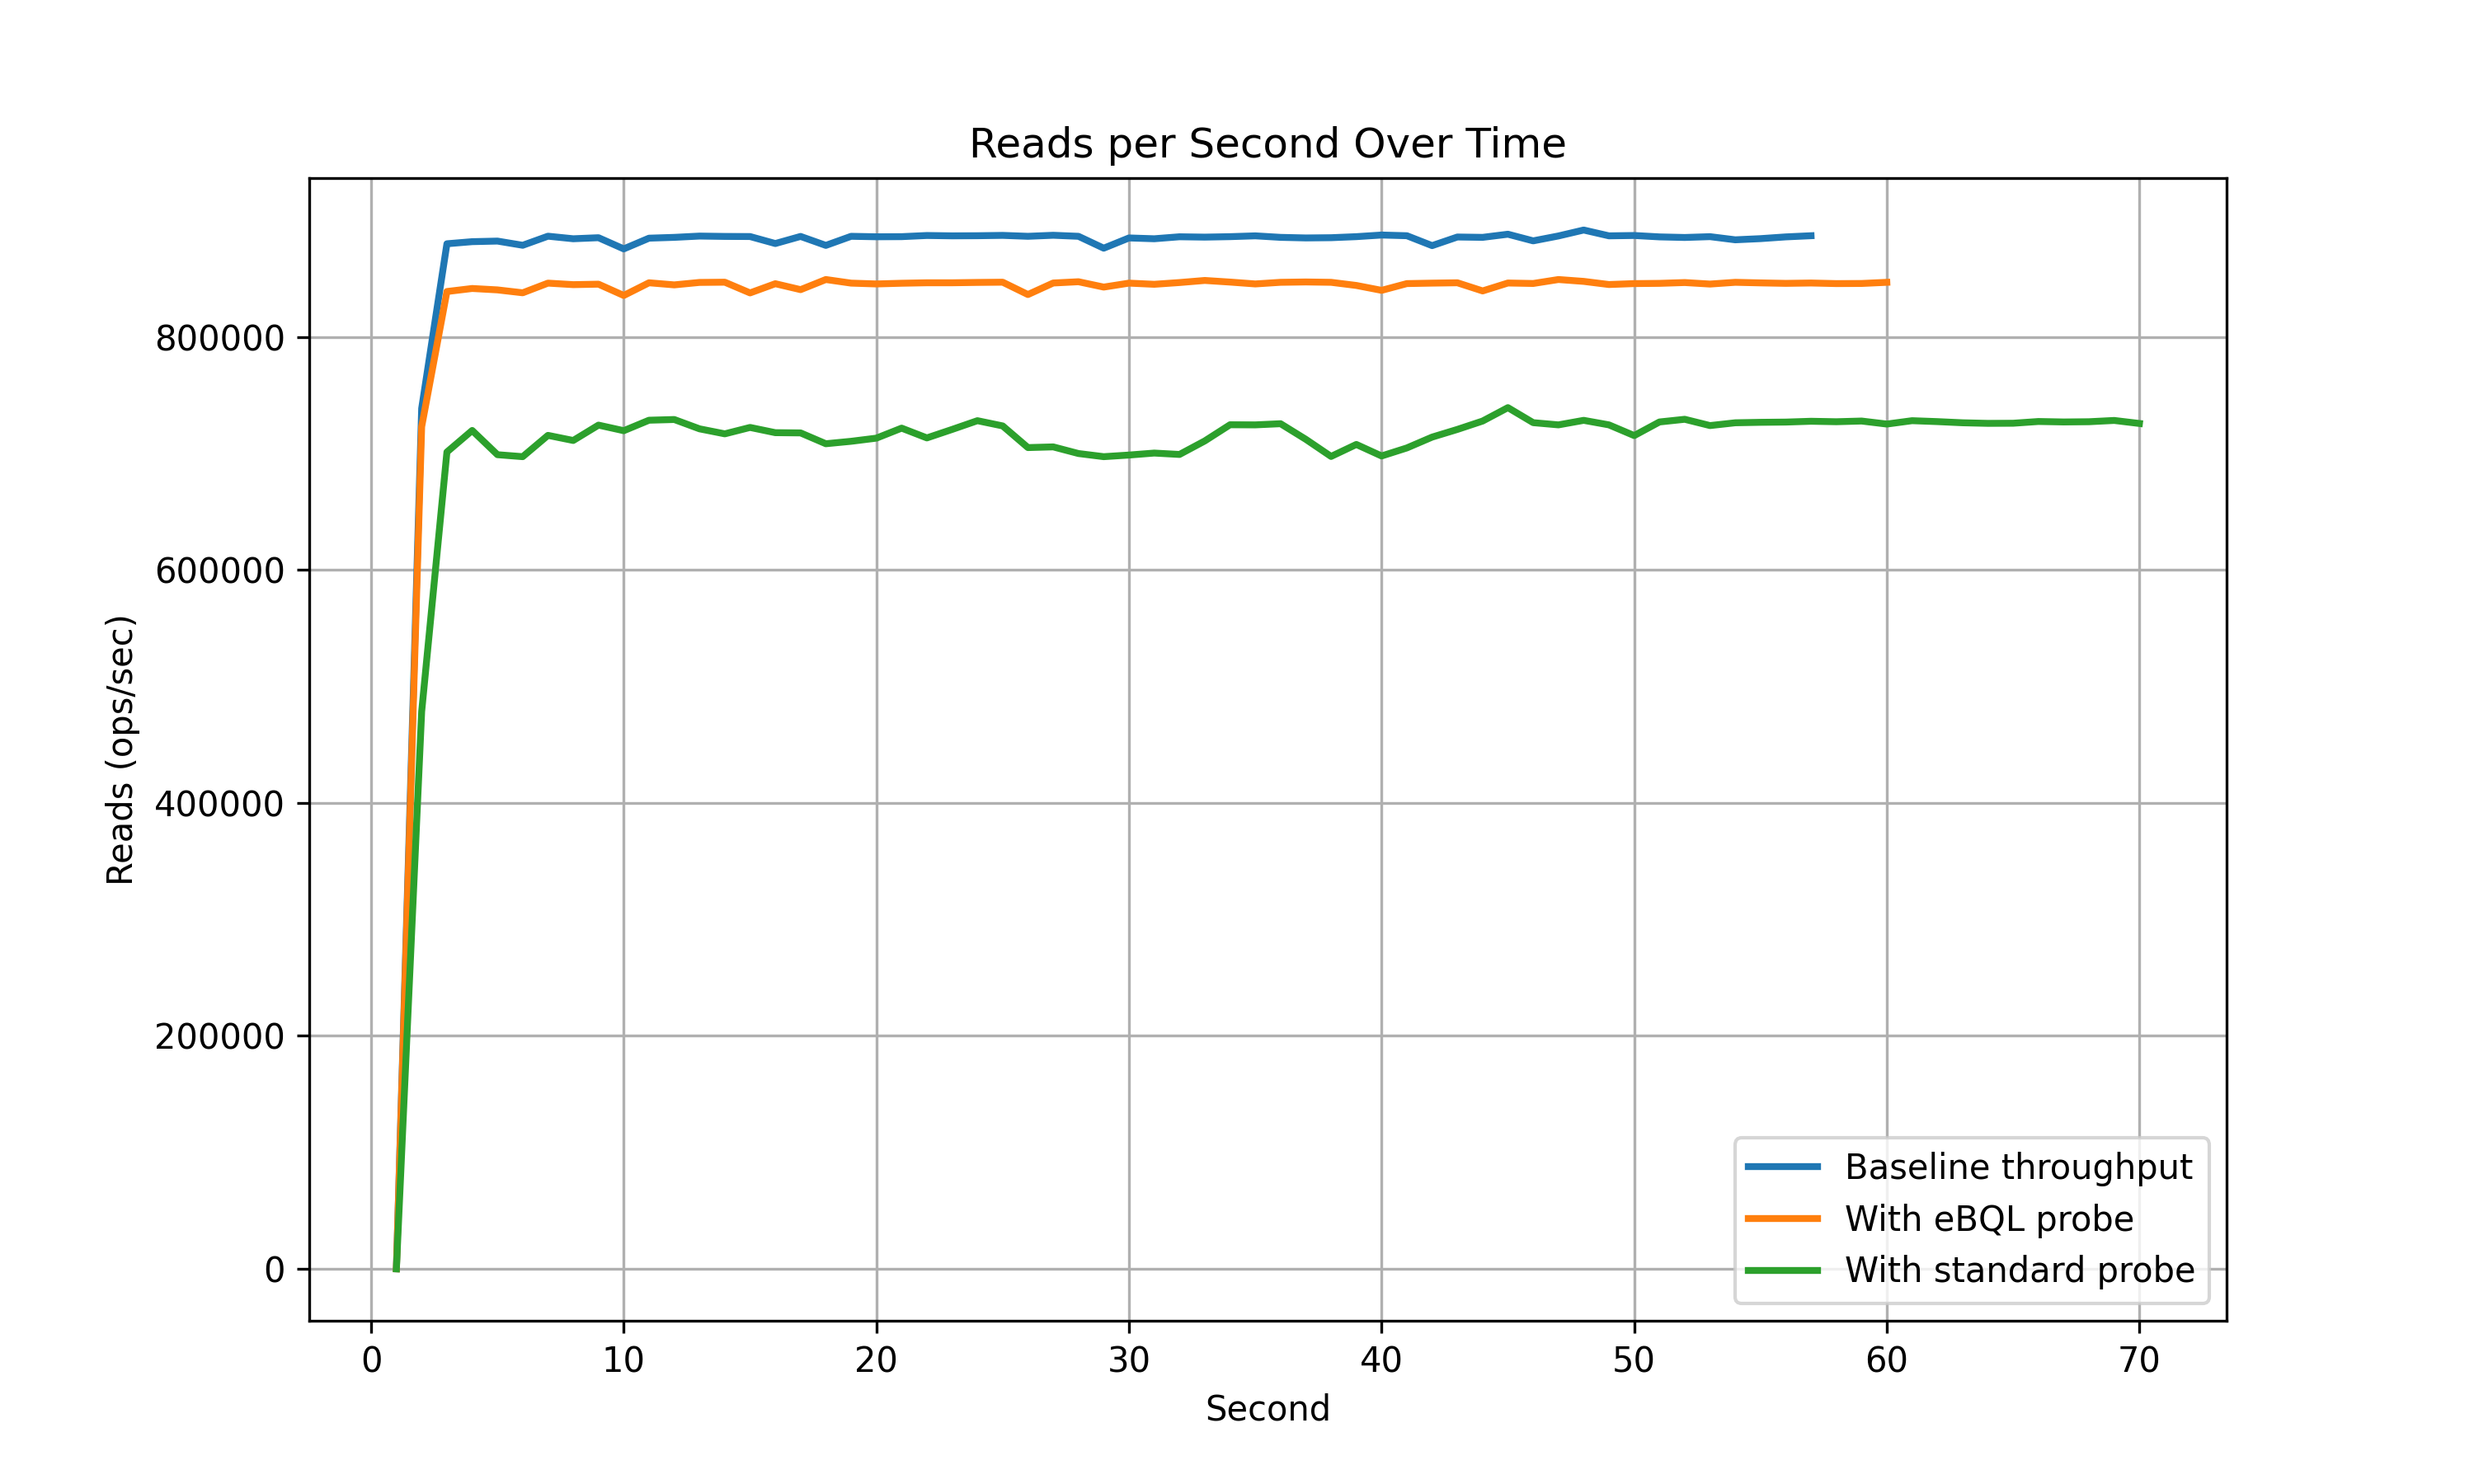
\includegraphics[width=\linewidth]{diagrams/baseline-eval-throughput-8.png}
        \caption{}
    \end{subfigure}
    \caption{End-to-end read throughput comparison on 12 (a) and 8 (b) CPUs.}
    \label{fig:baseline-eval-throughput}
\end{figure}

\subsection{Performance Drilldown}
\label{perf-drilldown}

We briefly investigate the cause behind standard probe's high overhead.

\begin{figure}
    \centering
    \begin{subfigure}{.8\textwidth}
        \centering
        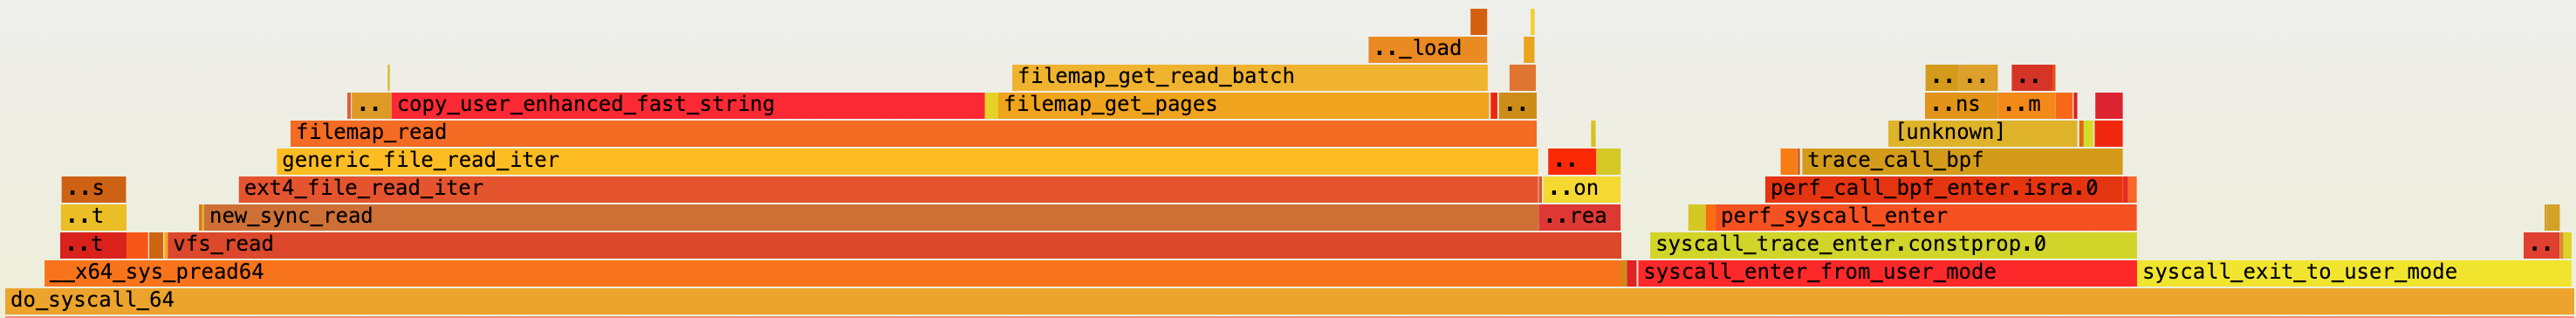
\includegraphics[width=\linewidth]{diagrams/opt-pread-fg.png}
        \caption{}
    \end{subfigure}

    \begin{subfigure}{.8\textwidth}
        \centering
        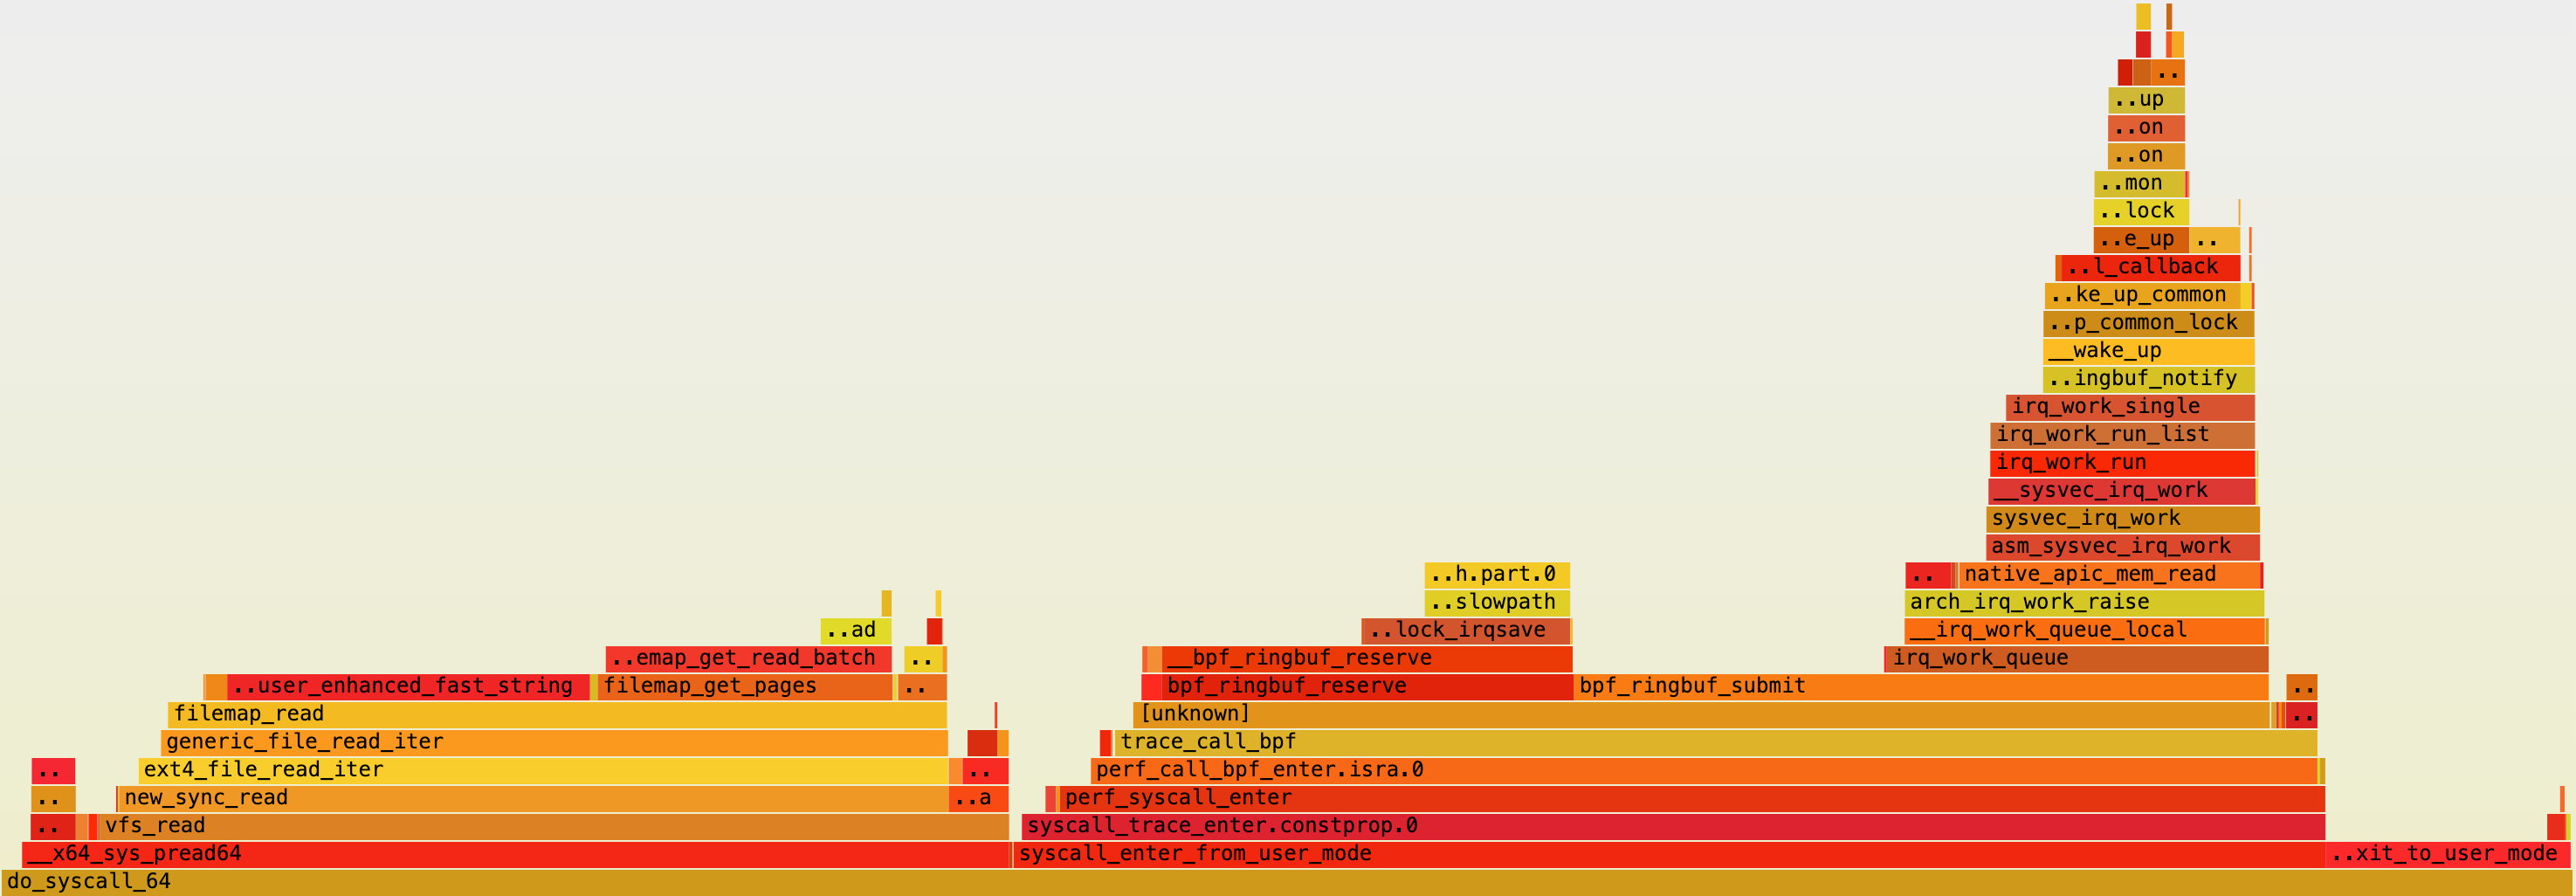
\includegraphics[width=\linewidth]{diagrams/unopt-pread-fg.png}
        \caption{}
    \end{subfigure}
    \caption{Flamegraphs of RocksDB's \texttt{pread64} syscall under the eBQL probe (a) and standard
    probe (b).}
    \label{fig:pread-fgs}
\end{figure}

Figure \ref{fig:pread-fgs} shows two flamegraphs comparing RocksDB's \texttt{do\_syscall\_64} stack
trace and rough execution proportions under an eBQL probe, and the standard probe. In the standard
probe, more than half the \texttt{pread64} syscall's time is spent in the BPF probe itself, in
particular reserving and submitting values to the BPF ring buffer to transmit values to user-space;
in contrast, only a small fraction of time is spent within the eBQL probe, with the two highest
overhead functions being hash map lookups and retrieving the \texttt{ktime}.

This also shows the BPF subsystem's overhead: in both programs, both entering the BPF program from
the syscall context and exiting the BPF program into user mode incur a non-trivial penalty (which
can be quantified from Table \ref{tab:baseline-eval-nums}).

\subsection{Discussion}

eBQL's probe itself, despite performing aggregations every time the window tumbles, manages to
maintain a low tail latency. On average, the probe runs for $\sim 160$ns, with around $\sim 120$ns
spent on infrastructure supporting the hook.

While eBQL is not a complete zero-cost abstraction, it only incurs minimal additional overhead over
the hand-optimized eBPF program, and provides significant performance improvements over a standard
eBPF probe that are only exacerbated in a resource-constrained environment. Further, in most cases,
the performance gap between eBQL and hand-optimized code is closeable. For instance, the key
optimization between eBQL and the hand-optimized code is utilizing per-CPU maps, since one of the
group-by keys was CPU. If eBQL's query optimizer can identify special cases to use per-CPU or
task-local storage, it is likely that eBQL probes can become on-par with hand-optimized code, with a
fraction of the development effort.


\section{Future Work}

eBQL is still a prototype; there is much future work left to explore.

We have shown that performing as much aggregation and filtering in kernel space significantly lowers
overhead by reducing the amount of data transmitted between to user space (\S \ref{perf-drilldown}).
Cost-based analysis and optimizations provide an opportunity to further develop this research: as
recent work starts to quantify performance characteristics (ref: in-kernel traffic sketching) and
latencies of specific BPF routines (ref: BPF runtime policy), it would be interesting to produce a
cost estimate based not on disk IO cost (as in traditional DBMSs), but rather specific BPF routines,
like kernel memory accesses or hash map iterations. Further, since BPF programs are executed
continuously, there is potential to gather statistics on data characteristics and use runtime flags
to dynamically enable/disable operators.

These cost-based optimizations become increasingly important as the Linux kernel supports more
features and gradually removes BPF restrictions. For instance, Linux v5.17 introduces an arbitrary
\texttt{bpf\_loop} that relaxes loop restrictions (ref: bpf-loop kernel patch), and Linux 6+
introduces \texttt{kfunc}s and non-BPF-map based data structures like linked lists and red-black
trees, opening the floor for performant dynamic memory (ref: kfuncs, rb trees). With these
constructs, joins can become feasible in kernel space, and so cost analysis to minimize tail
latencies becomes even more pertinent.

eBQL also adopts a relatively simple streaming approach that contains opportunities for
sophistication. Although BPF functions are event-based and thus cannot be manually scheduled, there
is opportunity to share synopses between multiple queries (e.g. if separate developers are querying
the same tracepoint), and there are various probabilistic sketch algorithms for efficient sub-linear
approximations that can be exploited. For instance, (ref: in-kernel traffic sketching) contains an
implementation of the count-min sketch; it would be interesting to investigate the performance and
\textit{feasibility} of other sketches, like HyperLogLog, Theta Sketches, and the t-digest/q-digest
for quantiles.

\section{Conclusion}

eBQL is an eBPF streaming query engine that facilitates performant HFT data collection via an
expressive interface, exposing a familiar relational layer over existing kernel tracing
infrastructure. eBQL eases the burden of understanding internal kernel/BPF infrastructure and
developing custom BPF programs, making low-overhead HFT data collection accessible to application
developers.

% References
\newpage
\bibliographystyle{plain}
\bibliography{references}
\addcontentsline{toc}{section}{References}

\newpage
\appendix

\section{Code Artifacts}
\label{app:ex-code}

The code for eBQL can be found at \texttt{https://github.com/ringtack/ebql}, and the benchmark code
can be found at \texttt{https://github.com/ringtack/ebql-benchmarks} (in particular, this contains
the optimized code used in \S \ref{opt-eval}).

\addcontentsline{toc}{section}{Appendix}

\end{document}
